\documentclass[12pt,a4paper]{article}

% ------------------------------------------------------------
% Packages
% ------------------------------------------------------------
\usepackage[utf8]{inputenc}
\usepackage[T1]{fontenc}
\usepackage{lmodern}
\usepackage{amsmath}
\usepackage{amssymb}
\usepackage{graphicx}
\usepackage{float}
\usepackage{geometry}
\usepackage{setspace}
\usepackage{parskip}
\usepackage{hyperref}

\geometry{
    margin=2.5cm
}

\onehalfspacing

% ------------------------------------------------------------
% Document
% ------------------------------------------------------------
\begin{document}

% =========================
% TITLE PAGE
% =========================

\begin{titlepage}
    \thispagestyle{empty}

    \centering

    \vspace*{3cm}

    {\Large \textsc{A Historical Development of Fluid Science}}\\[1.2cm]

    {\Huge \underline{\textbf{History of Fluid Mechanics, Meteorology}}}\\[0.35cm]
    {\Huge \underline{\textbf{and Physical Oceanography}}}\\[1.2cm]

    {\Large \textit{Important Scientists and Their Contributions}}\\[2.5cm]

    \rule{0.75\textwidth}{0.5pt}\\[1cm]

    {\large
    From Ancient Hydrostatics to Modern Fluid Dynamics\\
    and Physical Oceanography
    }\\[1cm]

    \rule{0.75\textwidth}{0.5pt}

    \vfill

    {\large
    \textbf{Fredrik Bergelv}\\[0.3cm]
    Course / University\\[0.3cm]
    \today
    }

\end{titlepage}

% Start page numbering from 1 on the next page
\pagenumbering{roman}
\setcounter{page}{1}

% ============================================================
% ARISTOTLE
% ============================================================
\section*{\underline{\textbf{Aristotle (384--322 BC)}}}

\textbf{Nationality:} Greek

\textbf{Generally known for:} Aristotle was one of the most influential philosophers of ancient Greece. His work covered physics, biology, logic, astronomy, ethics, politics, and natural philosophy.

\textbf{Contribution to fluid mechanics, meteorology and oceanography:}

Aristotle attempted to explain natural motion and the behaviour of fluids using observations of the physical world. In his work \textit{Meteorologica}, he discussed winds, clouds, rain, evaporation, water circulation, storms, and other atmospheric phenomena.

He proposed that water could be transformed into vapour by heating and later return as precipitation. Although his explanations were not based on modern thermodynamics, this was an early attempt to describe the atmosphere as part of a continuous physical cycle.

Aristotle also recognized that air and water behave differently from solid materials and discussed the resistance offered by a surrounding medium to moving objects. His ideas were qualitative rather than mathematical, but they helped establish the study of fluids and the atmosphere as subjects of natural philosophy.

\begin{figure}[H]
    \centering
    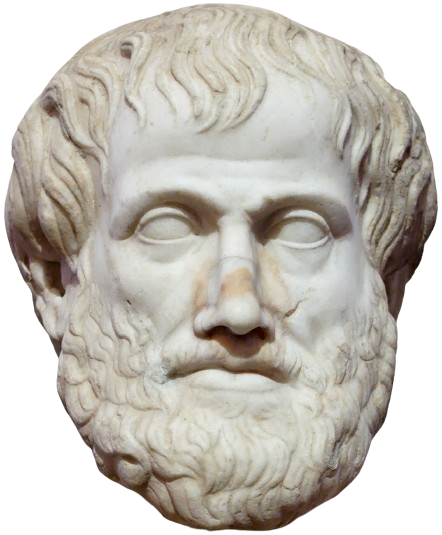
\includegraphics[width=0.30\textwidth]{Figures/Aristotle.png}
    \caption{Aristotle of Stagira}
\end{figure}


% ============================================================
% CTESIBIUS
% ============================================================
\newpage
\section*{\underline{\textbf{Ctesibius of Alexandria (c. 285--222 BC)}}}

\textbf{Nationality:} Greek, from Alexandria, Egypt

\textbf{Generally known for:} Ctesibius was an inventor and engineer who worked on pneumatics, water pumps, hydraulic machines, and mechanical devices.

\textbf{Contribution to fluid mechanics:}

Ctesibius was one of the first people to systematically exploit the mechanical behaviour of air and water. He developed improved piston pumps in which a piston moved inside a cylinder and forced water through valves. This demonstrated that a mechanical device could use pressure differences to transport water.

He also developed the hydraulic organ, which used water to regulate the pressure of air supplied to pipes. His work represents an important early connection between mechanical motion, pressure, and fluid flow.

Ctesibius also worked with compressed air. His experiments helped establish that air could be compressed and used to transmit mechanical forces, an idea that later became fundamental to pneumatics and fluid power.

\begin{figure}[H]
    \centering
    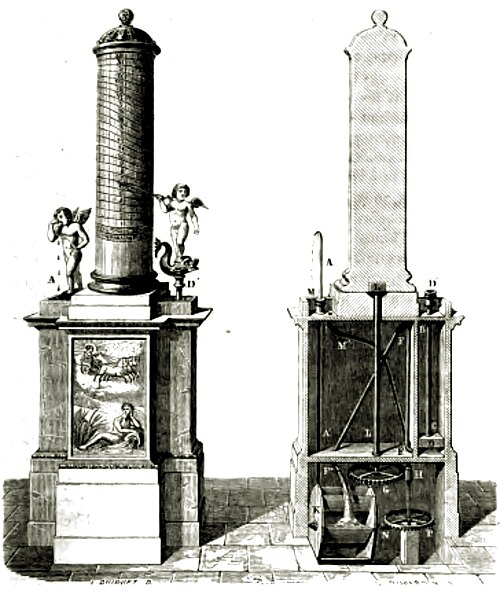
\includegraphics[width=0.40\textwidth]{Figures/Ctesibius.png}
    \caption{Ctesibius of Alexandrias water clock, illustrated by Claude Perrault.}
\end{figure}


% ============================================================
% ARCHIMEDES
% ============================================================
\newpage
\section*{\underline{\textbf{Archimedes of Syracuse (c. 287--212 BC)}}}

\textbf{Nationality:} Greek, from Syracuse in Sicily

\textbf{Generally known for:} Archimedes was a mathematician, physicist, engineer, astronomer, and inventor. He made major contributions to geometry, mechanics, centres of gravity, levers, and hydrostatics.

\textbf{Contribution to fluid mechanics:}

Archimedes established the foundations of hydrostatics through his study of fluids at rest and floating bodies. He did not know the modern differential equation for hydrostatic equilibrium, but his results can be reconstructed using the hydrostatic approximation. In a stationary fluid, the pressure gradient balances the weight of the fluid,

\[
\frac{dp}{dz}=-\rho_f g,
\]

where \(z\) is measured upward and \(\rho_f\) is the fluid density. This means that pressure increases with depth. The pressure acting on an immersed body is therefore greater on its deeper surfaces than on its shallower surfaces. The resulting pressure forces do not cancel, and their integration over the entire surface produces an upward buoyant force,

\[
F_B=\rho_f g V_{\mathrm{displaced}}.
\]

Archimedes also investigated the equilibrium and stability of floating bodies, making his work one of the earliest rigorous mathematical treatments of fluids at rest.

\begin{figure}[H]
    \centering
    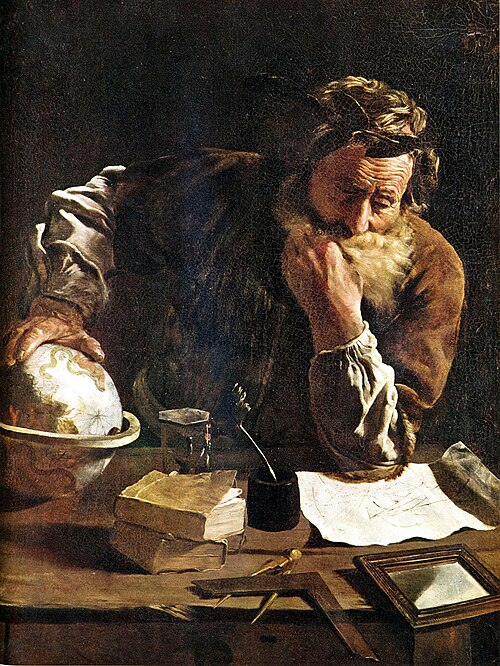
\includegraphics[width=0.30\textwidth]{Figures/Archimedes.png}
    \caption{Archimedes of Syracuse by Domenico Fetti.}
\end{figure}


% ============================================================
% HERO
% ============================================================
\newpage
\section*{\underline{\textbf{Hero of Alexandria (c. 10--70 AD)}}}

\textbf{Nationality:} Greek-Egyptian, from Alexandria

\textbf{Generally known for:} Hero was a mathematician, engineer, and inventor known for automatic machines, surveying instruments, pneumatics, and early steam-powered devices.

\textbf{Contribution to fluid mechanics:}

Hero investigated the behaviour of air and water in enclosed systems and designed machines that exploited pressure differences.

His \textit{Pneumatica} described devices using air pressure, water pressure, siphons, fountains, valves, and compressed air.

One of his most famous inventions was the aeolipile. Water was heated inside a vessel until steam escaped through bent nozzles. The escaping jets produced a reaction force that caused the vessel to rotate. Although the aeolipile was not developed into a practical steam engine, it demonstrated the mechanical effect of fluid jets.

Hero's work is particularly important because it connected fluid pressure, fluid discharge, and mechanical motion in practical machines.

\begin{figure}[H]
    \centering
    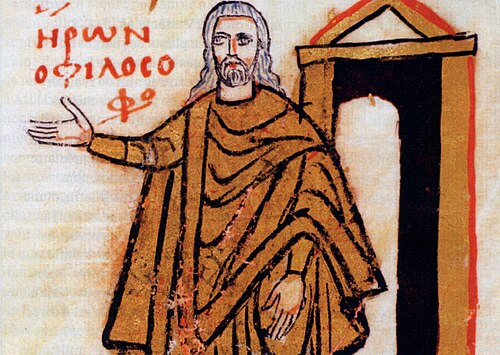
\includegraphics[width=0.40\textwidth]{Figures/Hero.png}
    \caption{\textit{Codex of Saint Gregory Nazianzus} including a drawing of Hero of Alexandria}
\end{figure}


% ============================================================
% HERO
% ============================================================
\newpage
\section*{\underline{\textbf{Ibn al-Haytham (c. 965--c. 1040)}}}

\textbf{Nationality:} Iraqi, born in Basra and later worked in Cairo.

\textbf{Generally known for:} Optics, mathematics, astronomy, and pioneering the experimental method in science. He is especially famous for his \textit{Book of Optics}, his experiments on reflection, refraction, vision, and the camera obscura.

\textbf{Contribution to fluid mechanics:}
Ibn al-Haytham studied the atmosphere as a physical medium and investigated how it affects the path of light. By studying atmospheric refraction and using geometrical reasoning, he made an early quantitative estimate of the height or thickness of the atmosphere. 

Although his estimate was based on simplified assumptions and differs greatly from the modern structure of the atmosphere, it was significant because he attempted to determine a physical property of the atmosphere from observable effects. His work therefore represents an early connection between geometry, observation, and the physical study of the atmosphere, preceding the later quantitative development of atmospheric and fluid science.

\begin{figure}[H]
    \centering
    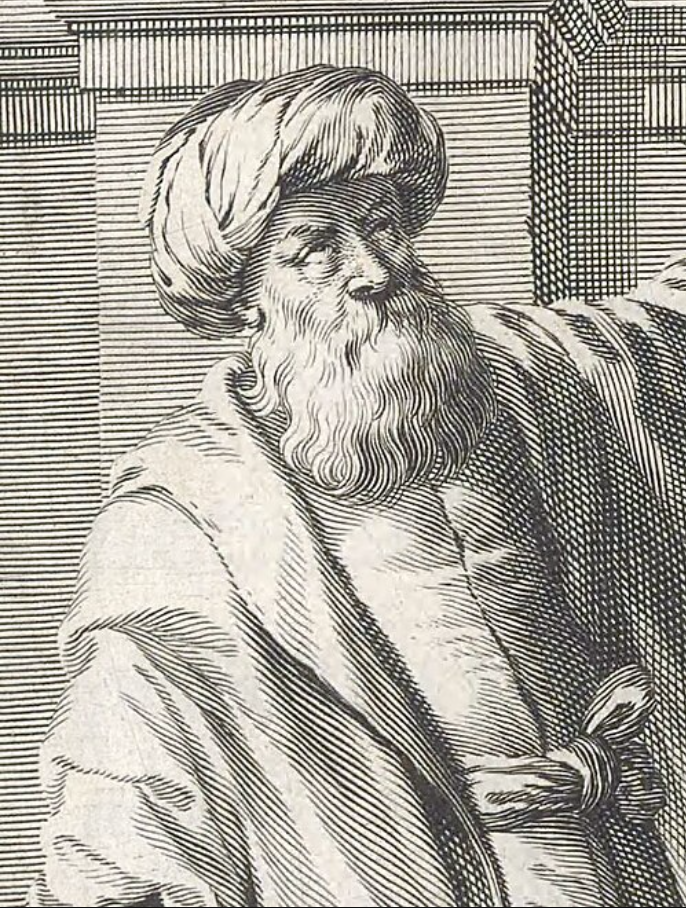
\includegraphics[width=0.30\textwidth]{Figures/Alhazen.png}
    \caption{Ibn al-Haytham by Jeremias Falck}
\end{figure}


% ============================================================
% LEONARDO
% ============================================================
\newpage
\section*{\underline{\textbf{Leonardo da Vinci (1452--1519)}}}

\textbf{Nationality:} Italian

\textbf{Generally known for:} Leonardo was a painter, engineer, anatomist, inventor, architect, and scientist.

\textbf{Contribution to fluid mechanics:}

Leonardo made remarkably detailed observations of moving water. He studied rivers, channels, waves, eddies, vortices, jets, hydraulic jumps, and the motion of water around obstacles.

He drew observations of water flowing through channels and recognized that turbulence contains complicated rotating structures. He also observed that water issuing from an opening forms a jet whose shape changes as it falls.

Leonardo investigated the relationship between the width and depth of flowing channels and the amount of water transported. He also studied waves and recognized that wave motion can propagate through water without the water particles themselves travelling with the wave over long distances.

His notebooks contain some of the earliest detailed scientific drawings of turbulent flow and hydraulic phenomena.

\begin{figure}[H]
    \centering
    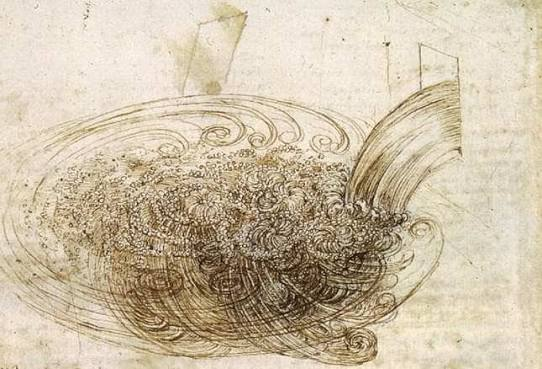
\includegraphics[width=0.50\textwidth]{Figures/Leonardo.png}
    \caption{Water falling upon water by Leonardo da Vinci}
\end{figure}


% ============================================================
% SIMON STEVIN
% ============================================================
\newpage
\section*{\underline{\textbf{Simon Stevin (1548--1620)}}}

\textbf{Nationality:} Flemish

\textbf{Generally known for:} Stevin was a mathematician, engineer, and scientist known for his work in statics, mathematics, engineering, and decimal notation.

\textbf{Contribution to fluid mechanics:}

Stevin developed an early mathematical theory of hydrostatics. He demonstrated that pressure in a fluid increases with depth and recognized that the pressure at a given depth depends on the depth and density of the fluid rather than the shape of the container.

This is expressed today as

\[
p=p_0+\rho gh.
\]

This idea is sometimes illustrated with Stevin's ``hydrostatic paradox'': containers with very different shapes can produce the same pressure at the same depth.

Stevin's work helped establish the concept that fluid pressure is a local property of the fluid and does not simply depend on the total amount of fluid contained in a vessel.

\begin{figure}[H]
    \centering
    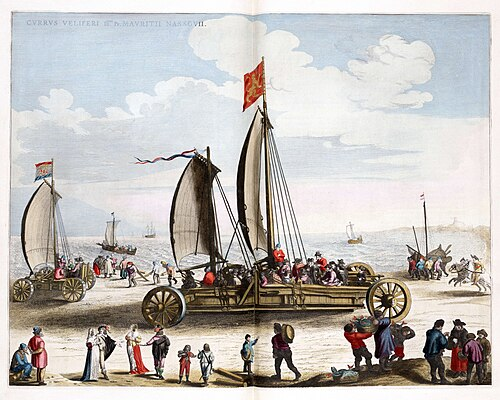
\includegraphics[width=0.45\textwidth]{Figures/Stevin.png}
    \caption{Wind chariot or land yacht designed by Simon Stevin}
\end{figure}


% ============================================================
% GALILEO
% ============================================================
\newpage
\section*{\underline{\textbf{Galileo Galilei (1564--1642)}}}

\textbf{Nationality:} Italian

\textbf{Generally known for:} Galileo was an astronomer, physicist, mathematician, and engineer. He is famous for telescopic astronomy, studies of falling bodies, inertia, projectile motion, and experimental physics.

\textbf{Contribution to fluid mechanics:}

Galileo studied the behaviour of bodies immersed in fluids, especially the problem of why some objects float while others sink. He examined density and specific gravity and investigated floating bodies experimentally. His work challenged older explanations of buoyancy and helped move the subject toward quantitative measurement.

A particularly important problem was the apparent paradox of a heavy ship floating while a small piece of the same material sinks. Galileo's analysis helped establish that floating depends on the relationship between the body's weight and the hydrostatic forces acting on it, rather than simply on whether the material itself is heavier than water. His work also contributed to the experimental approach that later became central to fluid mechanics.

\begin{figure}[H]
    \centering
    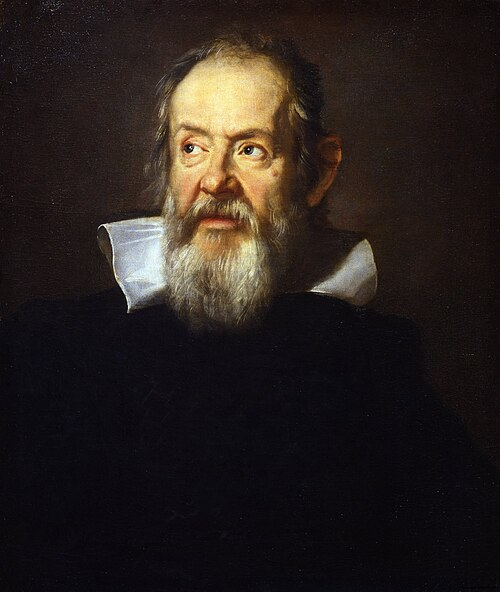
\includegraphics[width=0.30\textwidth]{Figures/Galileo.png}
    \caption{Galileo Galilei}
\end{figure}

% ============================================================
% OTTO VON GUERICKE
% ============================================================
\newpage
\section*{\underline{\textbf{Otto von Guericke (1602--1686)}}}

\textbf{Nationality:} German

\textbf{Generally known for:} Von Guericke was a physicist, engineer, inventor, and mayor of Magdeburg. He is famous for experiments with vacuum and atmospheric pressure.

\textbf{Contribution to fluid mechanics and atmospheric science:}

Von Guericke constructed one of the first effective air pumps and used it to investigate what happens when air is removed from a vessel. His most famous demonstration involved the Magdeburg hemispheres. Two metal hemispheres were joined and the air inside was pumped out. Teams of horses were unable to pull the hemispheres apart. Once air was allowed back inside, they could be separated easily.

The experiment demonstrated the enormous mechanical effect of atmospheric pressure. If the pressure difference across an area is \(\Delta p\), the resulting force is approximately

\[
F=\Delta p A.
\]

Von Guericke's experiments provided powerful experimental evidence that air exerts pressure and that atmospheric pressure is a real mechanical force.

\begin{figure}[H]
    \centering
    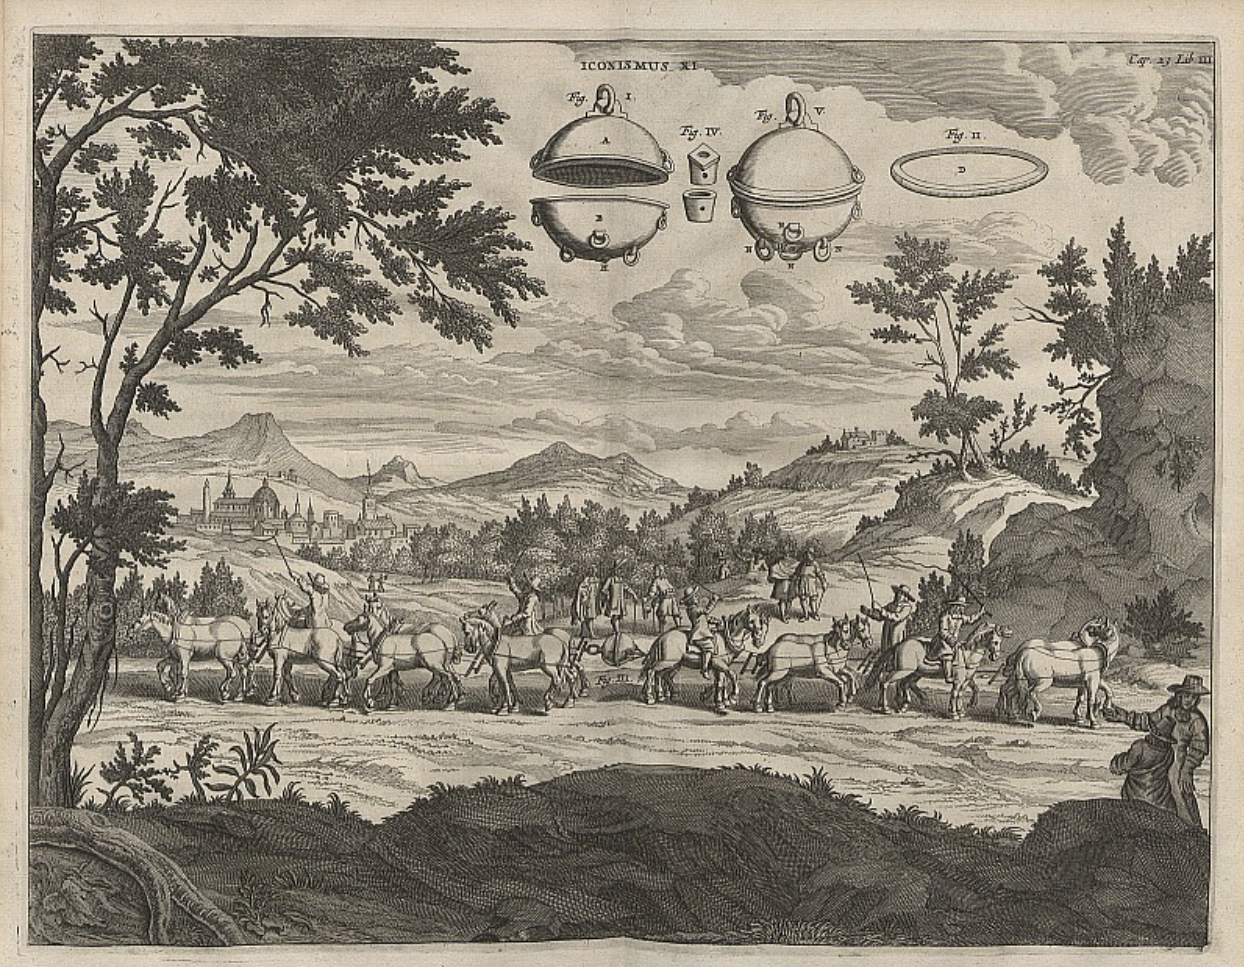
\includegraphics[width=0.50\textwidth]{Figures/Guericke.png}
    \caption{Gaspar Schott's sketch of Otto von Guericke's Magdeburg hemispheres experiment}
\end{figure}


% ============================================================
% TORRICELLI
% ============================================================
\newpage
\section*{\underline{\textbf{Evangelista Torricelli (1608--1647)}}}

\textbf{Nationality:} Italian

\textbf{Generally known for:} Torricelli was a mathematician and physicist, student of Galileo, and inventor of the mercury barometer.

\textbf{Contribution to fluid mechanics:}

Torricelli studied the speed at which a liquid leaves a tank through a small opening.

For a tank with a free surface at height \(h\) above the opening, he derived the result

\[
v=\sqrt{2gh} \implies v\propto\sqrt{h}.
\]
The result shows that the exit velocity is related to the conversion of gravitational potential energy into kinetic energy. It is an early form of what is now recognized as a Bernoulli-type energy relation.

Torricelli also invented the mercury barometer. A long glass tube was filled with mercury, inverted into a reservoir, and left with a vacuum above the mercury column. Atmospheric pressure supporting the mercury produced the barometric height.

The relation is

\[
p_{\mathrm{atm}}=\rho_{\mathrm{Hg}}gh.
\]

This connected atmospheric pressure to a measurable height and became fundamental to meteorology.

\begin{figure}[H]
    \centering
    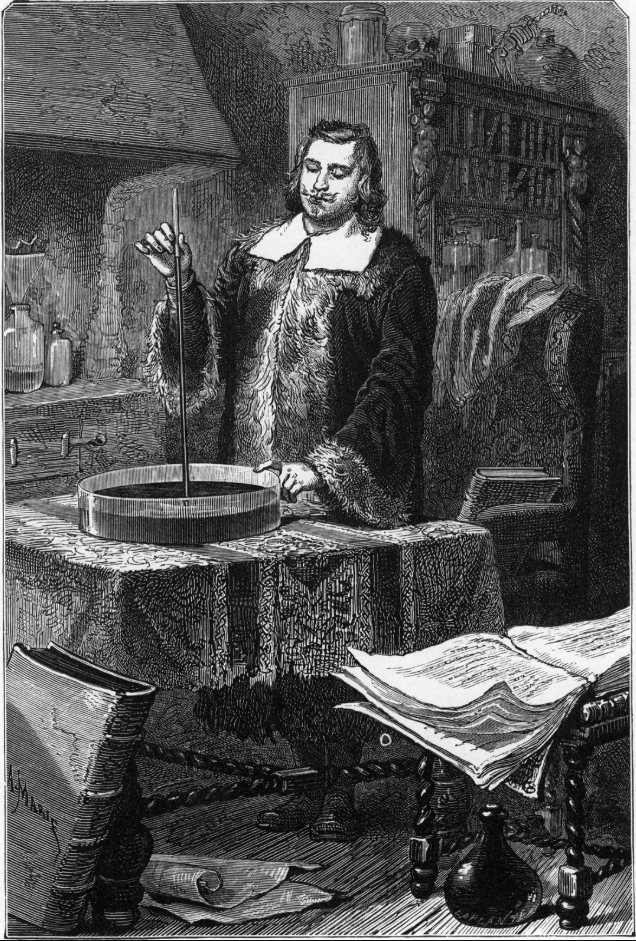
\includegraphics[width=0.3\textwidth]{Figures/Torricelli.png}
    \caption{Evangelista Torricelli}
\end{figure}


% ============================================================
% PASCAL
% ============================================================
\section*{\underline{\textbf{Blaise Pascal (1623--1662)}}}

\textbf{Nationality:} French

\textbf{Generally known for:} Pascal was a mathematician, physicist, philosopher, inventor, and theologian. He made major contributions to mathematics, probability theory, and the study of pressure and fluids.

\textbf{Contribution to fluid mechanics:}

Pascal investigated atmospheric pressure and how pressure is transmitted through fluids. His experiments helped establish that the atmosphere exerts pressure because of the weight of the air above us. In 1648, his brother-in-law Florin Périer carried out Pascal's famous experiment on the Puy de Dôme, measuring the height of a mercury column at different elevations. The mercury column became shorter at higher altitude, showing that atmospheric pressure decreases with height.

Pascal also used a simple but striking argument involving a long tube filled with wine. If a tube is inverted into a container of wine, the atmosphere can support the column of liquid, but only up to a certain height. For a liquid column in hydrostatic equilibrium, gives a maximum height of roughly \(10\)--\(11\,\mathrm{m}\) under normal atmospheric pressure. This was an important demonstration that it is the atmosphere pushing the liquid upward, rather than the act of ``suction'' pulling the liquid upward.

Pascal also established the principle now known as Pascal's law: a pressure change applied to a confined fluid is transmitted throughout the fluid. Since pressure is force over area one obtains: 
\[
\frac{F_1}{A_1}=\frac{F_2}{A_2}.
\]

These experiments and principles made Pascal one of the key figures in the development of hydrostatics and the understanding of atmospheric pressure.

\begin{figure}[H]
    \centering
    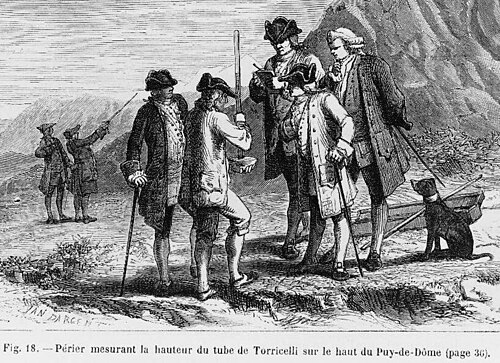
\includegraphics[width=0.50\textwidth]{Figures/Pascal.png}
    \caption{Florin Périer on the Puy de Dôme}
\end{figure}


% ============================================================
% BOYLE
% ============================================================
\newpage
\section*{\underline{\textbf{Robert Boyle (1627--1691)}}}

\textbf{Nationality:} Irish

\textbf{Generally known for:} Boyle was a physicist, chemist, and natural philosopher. He is often considered one of the founders of modern chemistry.

\textbf{Contribution to fluid mechanics and gas physics:}

Boyle used air pumps to investigate the relationship between pressure and volume. For a fixed quantity of gas at approximately constant temperature, he found that pressure increases as volume decreases:

\[
pV=\text{constant}.
\]

Therefore,

\[
p\propto\frac{1}{V}.
\]

This became known as Boyle's law.

His experiments showed that air is compressible and that pressure and volume are quantitatively related. This was an important step toward treating gases mathematically rather than simply as invisible substances with qualitative properties.

\begin{figure}[H]
    \centering
    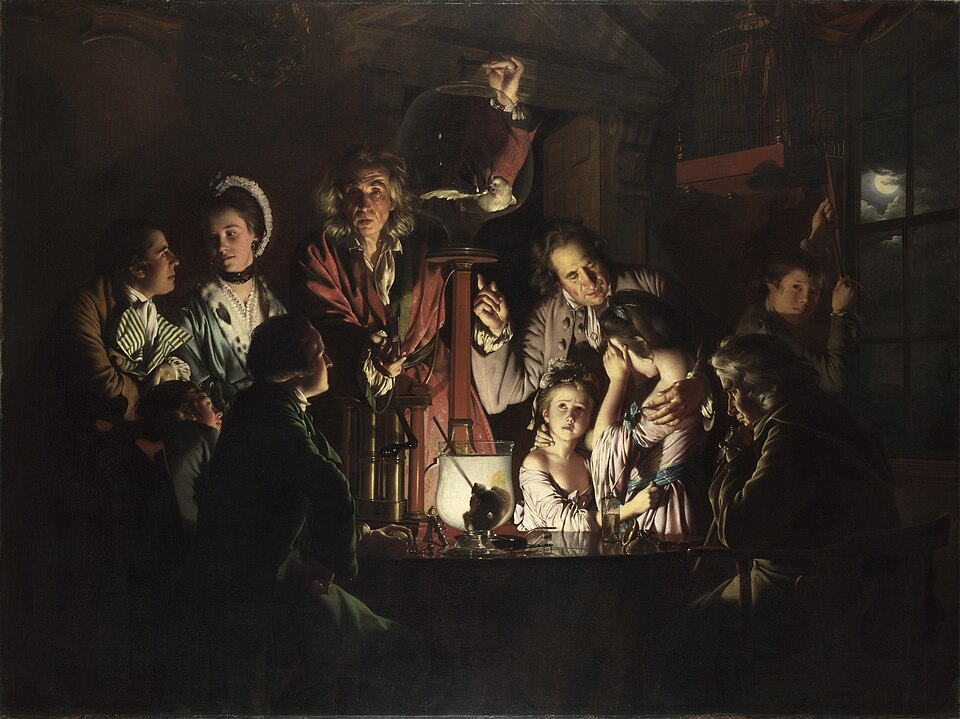
\includegraphics[width=0.50\textwidth]{Figures/Boyle.png}
    \caption{\textit{An Experiment on a Bird in the Air Pump} by Joseph Wright of Derby, displaying Robert Boyle}
\end{figure}


% ============================================================
% MARIOTTE
% ============================================================
\newpage
\section*{\underline{\textbf{Edme Mariotte (c. 1620--1684)}}}

\textbf{Nationality:} French

\textbf{Generally known for:} Mariotte was a physicist and natural philosopher who worked on mechanics, optics, plant physiology, and atmospheric phenomena.

\textbf{Contribution to fluid mechanics and gas physics:}

Mariotte independently investigated the relationship between pressure and volume in gases. For a fixed amount of gas at constant temperature,

\[
pV=\text{constant}.
\]

Thus,

\[
p\propto\frac{1}{V}.
\]

His experiments helped establish what became known as Boyle's law in the English-speaking world and Boyle--Mariotte's law in many European countries.

Mariotte also studied the behaviour of air and water and contributed to the growing experimental tradition of measuring physical quantities rather than relying only on philosophical arguments.

%\begin{figure}[H]
    %\centering
    %\includegraphics[width=0.30\textwidth]{Figures/Mariotte.png}
    %\caption{Edme Mariotte}
%\end{figure}


% ============================================================
% HOOKE
% ============================================================
\newpage
\section*{\underline{\textbf{Robert Hooke (1635--1703)}}}

\textbf{Nationality:} English

\textbf{Generally known for:} Hooke was a physicist, mathematician, astronomer, microscopist, architect, and inventor. He is famous for Hooke's law of elasticity and his book \textit{Micrographia}.

\textbf{Contribution to fluid mechanics and gas physics:}

Hooke developed an early microscopic explanation of the behaviour of gases and thermal expansion. He proposed that air consists of very small particles in continual motion and that the impacts of these particles against surfaces produce air pressure. This is an important qualitative precursor to the kinetic theory of gases.

He also proposed that heating matter changes the motion of its microscopic particles. Increased molecular motion could cause particles to separate farther apart, explaining the expansion of matter when heated.

This idea is particularly important because it connected temperature and heat with microscopic motion rather than treating heat as a separate material substance.

Hooke's ideas therefore anticipated two major concepts of later physics:
\[
\text{gas pressure} \longleftrightarrow \text{microscopic particle motion},
\]
\[
\implies \text{thermal expansion} \longleftrightarrow \text{increased microscopic motion}.
\]
These ideas later became central to kinetic theory and thermodynamics.

\begin{figure}[H]
    \centering
    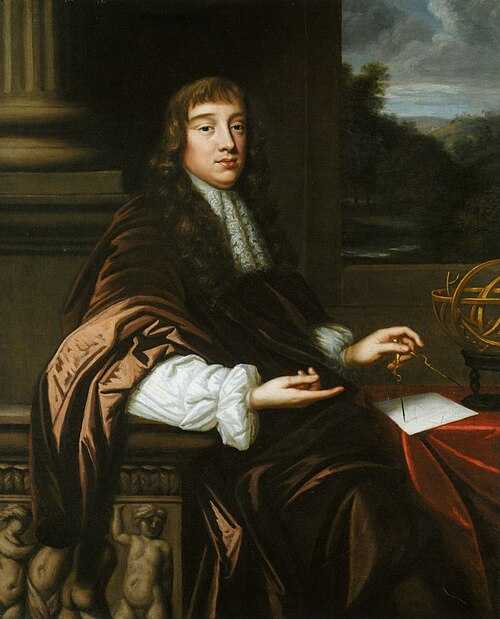
\includegraphics[width=0.30\textwidth]{Figures/Hooke.png}
    \caption{Portrait of a Mathematician by Mary Beale, could be Hooke}
\end{figure}


% ============================================================
% NEWTON
% ============================================================
\newpage
\section*{\underline{\textbf{Isaac Newton (1643--1727)}}}

\textbf{Nationality:} English

\textbf{Generally known for:} Newton was a mathematician, physicist, astronomer, and natural philosopher. He developed the laws of motion and universal gravitation and made major contributions to optics and calculus.

\textbf{Contribution to fluid mechanics:}

Newton established the mathematical framework for applying forces to moving fluids. His second law,

\[
\mathbf{F}=m\mathbf{a},
\]

provides the basic momentum equation from which fluid dynamics can be developed.

Newton also investigated the resistance and internal friction of fluids. For a Newtonian fluid, the shear stress is proportional to the velocity gradient:

\[
\tau=\mu\frac{du}{dy} \implies \tau\propto\frac{du}{dy}.
\]

Here \(\mu\) is the dynamic viscosity. This relationship is the defining constitutive relation for a Newtonian fluid and remains fundamental to modern fluid mechanics.

Newton also studied the motion of fluids in his \textit{Principia}, including the resistance experienced by bodies moving through fluids.

\begin{figure}[H]
    \centering
    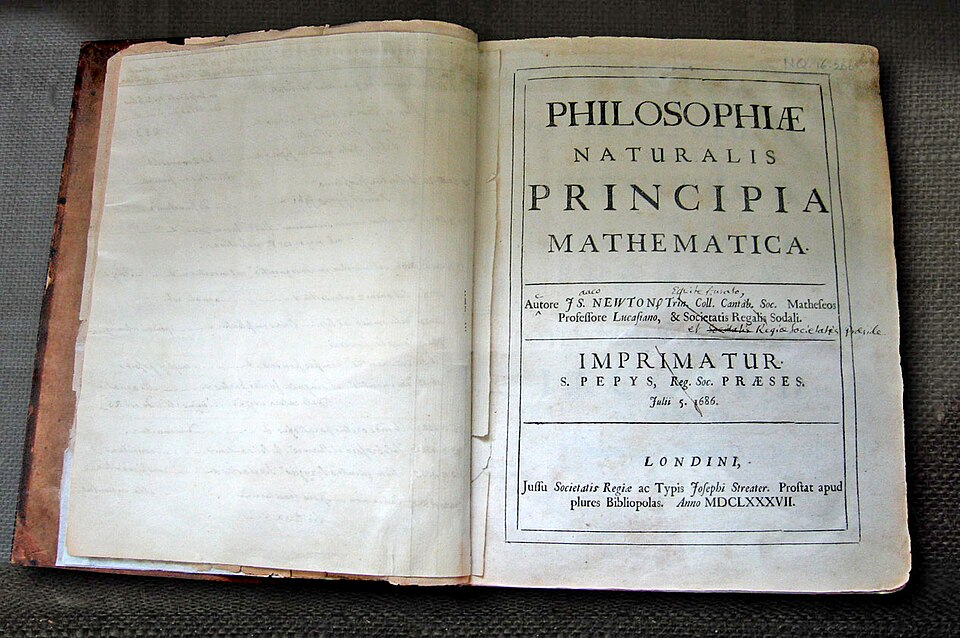
\includegraphics[width=0.45\textwidth]{Figures/Newton.png}
    \caption{Isaac Newtons \textit{Principia}}
\end{figure}


% ============================================================
% HALLEY
% ============================================================
\newpage
\section*{\underline{\textbf{Edmond Halley (1656--1742)}}}

\textbf{Nationality:} English

\textbf{Generally known for:} Halley was an astronomer, mathematician, physicist, meteorologist, and navigator. He is famous for calculating the orbit of Halley's Comet.

\textbf{Contribution to meteorology and physical oceanography:}

Halley made one of the earliest serious attempts to describe global atmospheric circulation using observations. During his time on the island of St.~Helena, he carefully observed the prevailing winds. He recorded that winds repeatedly came from characteristic directions rather than changing randomly from one direction to another. He used these observations, together with reports from other parts of the world, to construct an early global map of prevailing winds.

Halley proposed that solar heating was responsible for the large-scale circulation of the atmosphere. He suggested that stronger heating near the equator causes air to rise, with surrounding air moving toward the heated region. Although the circulation mechanism he proposed was incomplete, the important step was methodological: Halley attempted to combine observations from different parts of the world into a global physical model of atmospheric circulation.

\begin{figure}[H]
    \centering
    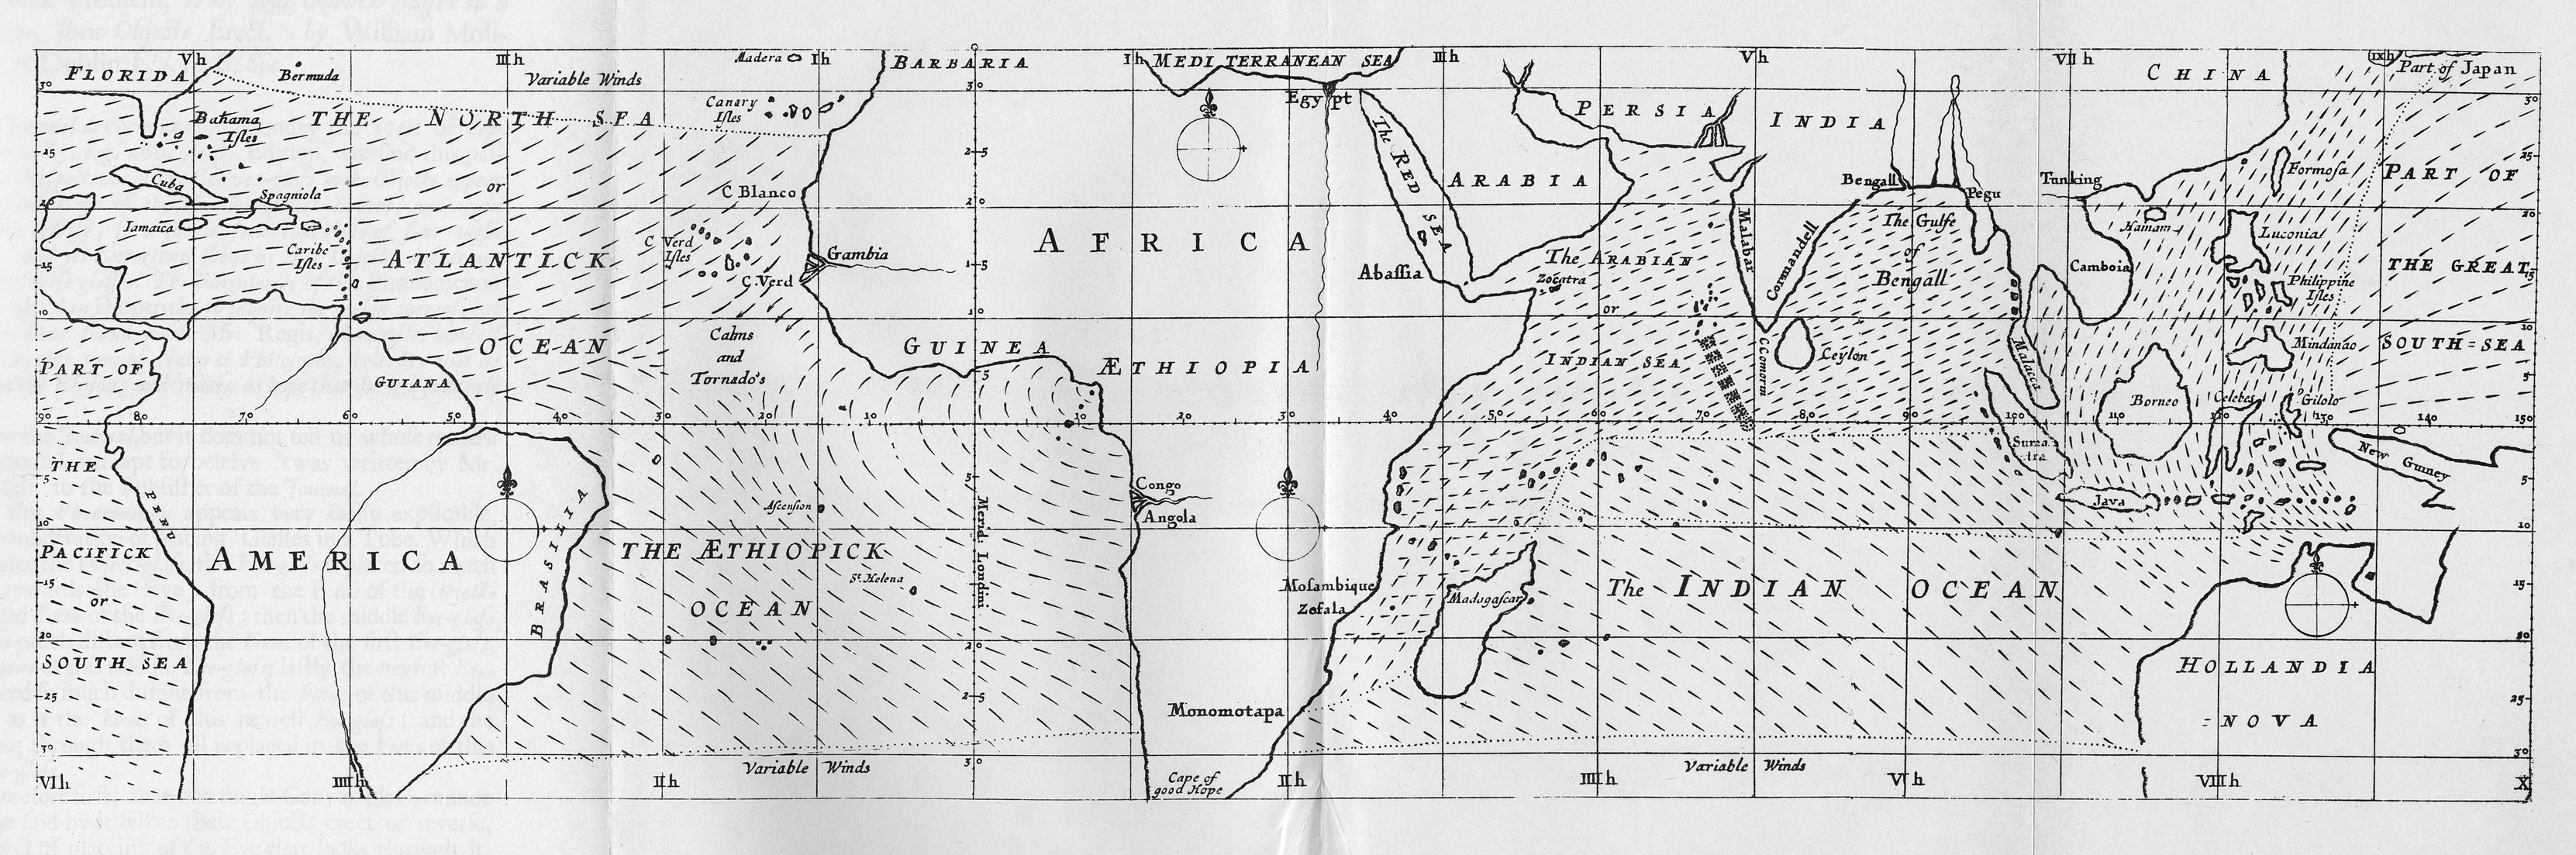
\includegraphics[width=0.90\textwidth]{Figures/Halley.png}
    \caption{Edmond Halleys map showing large scale circulation}
\end{figure}


% ============================================================
% HADLEY
% ============================================================
\newpage
\section*{\underline{\textbf{George Hadley (1685--1768)}}}

\textbf{Nationality:} English

\textbf{Generally known for:} Hadley was a lawyer, mathematician, and meteorologist.

\textbf{Contribution to meteorology:}

Hadley provided the first convincing physical explanation of the trade winds in terms of the Earth's rotation. He proposed that air heated near the equator rises and flows poleward at high altitude. Because the Earth rotates beneath the moving air, the air acquires an apparent east-west deflection.

In modern terms, the horizontal Coriolis acceleration is

\[
f=2\Omega\sin\phi,
\]

where \(\Omega\) is the Earth's rotation rate and \(\phi\) is latitude.

Hadley's work was therefore an early recognition that atmospheric circulation cannot be explained by heating alone: Earth's rotation changes the direction of large-scale winds. The circulation pattern associated with this idea is now called the Hadley circulation.

%\begin{figure}[H]
    %\centering
    %\includegraphics[width=0.30\textwidth]{Figures/George_Hadley.png}
    %\caption{George Hadley}
%\end{figure}


% ============================================================
% DANIEL BERNOULLI
% ============================================================
\newpage
\section*{\underline{\textbf{Daniel Bernoulli (1700--1782)}}}

\textbf{Nationality:} Swiss

\textbf{Generally known for:} Daniel Bernoulli was a mathematician and physicist and a member of the famous Bernoulli family. He worked in mathematics, probability, mechanics, and hydrodynamics.

\textbf{Contribution to fluid mechanics:}

Bernoulli developed one of the most important energy relationships in fluid mechanics.

For steady, incompressible, inviscid flow along a streamline,

\[
p+\frac{1}{2}\rho v^2+\rho gz=\text{constant}.
\]

The three terms represent pressure energy per unit volume, kinetic energy per unit volume, and gravitational potential energy per unit volume.

The equation shows that if the elevation remains approximately constant, an increase in flow speed is associated with a decrease in static pressure:

\[
p+\frac{1}{2}\rho v^2=\text{constant}.
\]

Bernoulli used this type of reasoning to connect fluid pressure and velocity.

His work helped transform fluid mechanics from a collection of hydrostatic observations into a mathematical science based on conservation laws.

\begin{figure}[H]
    \centering
    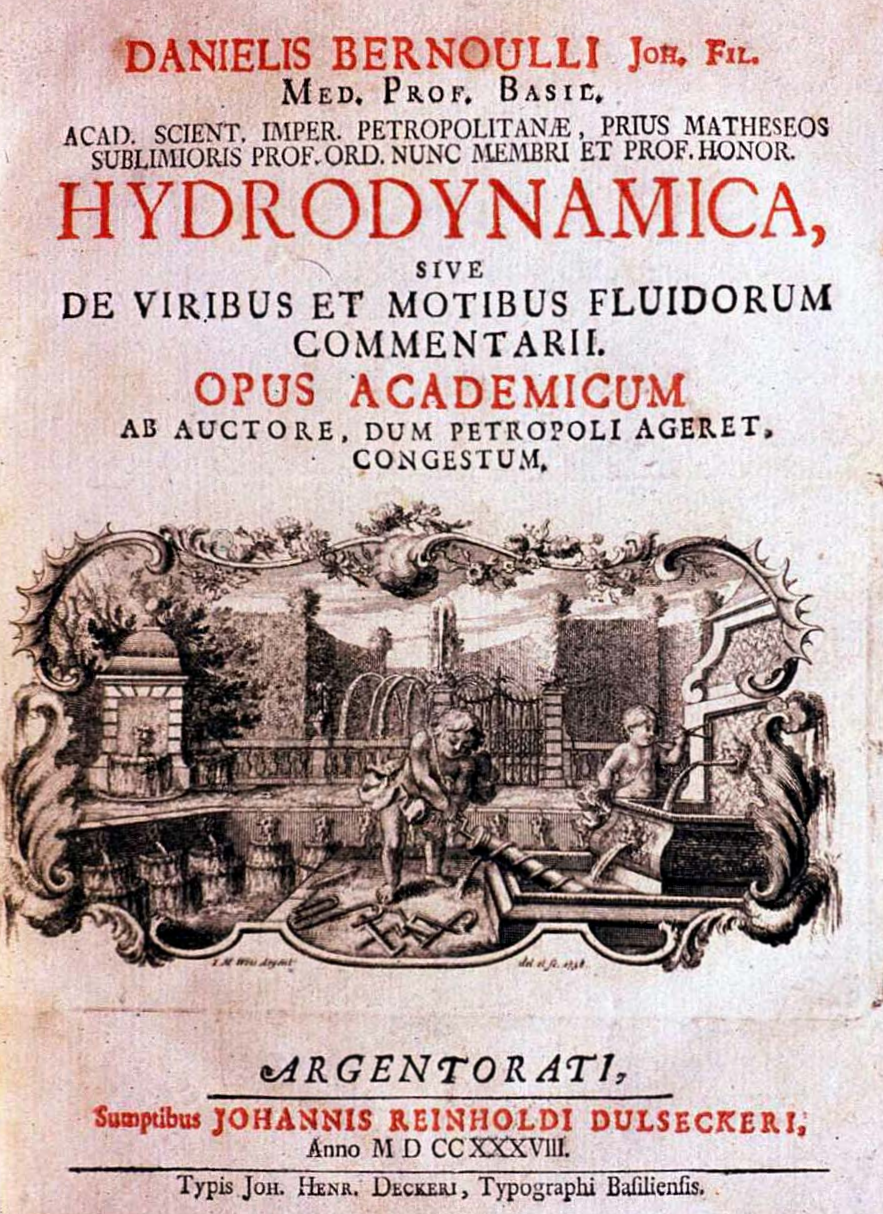
\includegraphics[width=0.30\textwidth]{Figures/Bernoulli.png}
    \caption{\textit{Hydrodynamica} by Daniel Bernoulli}
\end{figure}


% ============================================================
% EULER
% ============================================================
\newpage
\section*{\underline{\textbf{Leonhard Euler (1707--1783)}}}

\textbf{Nationality:} Swiss

\textbf{Generally known for:} Euler was one of the most prolific mathematicians in history. He contributed to calculus, differential equations, number theory, mechanics, astronomy, and mathematical physics.

\textbf{Contribution to fluid mechanics:}

Euler formulated the differential equations governing ideal fluid motion. For an inviscid fluid, the momentum equation can be written as

\[
\rho\left(
\frac{\partial \mathbf{u}}{\partial t}
+
\mathbf{u}\cdot\nabla\mathbf{u}
\right)
=
-\nabla p+\rho\mathbf{g}.
\]

These are now called the Euler equations. Euler's equations describe the acceleration of a fluid resulting from pressure gradients and body forces when viscosity is neglected.

Euler also introduced the modern mathematical description of fluid velocity as a field,

\[
\mathbf{u}=\mathbf{u}(\mathbf{x},t),
\]

allowing fluid motion to be described mathematically at every point in space and time.

\begin{figure}[H]
    \centering
    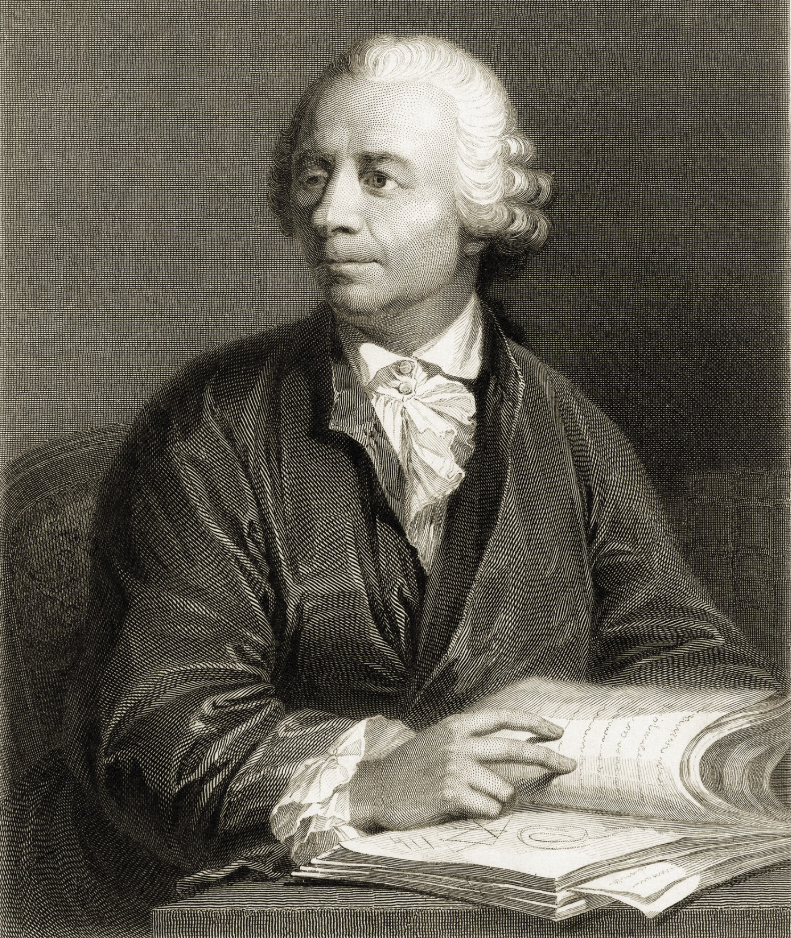
\includegraphics[width=0.30\textwidth]{Figures/Euler.png}
    \caption{Leonhard Euler}
\end{figure}


% ============================================================
% D'ALEMBERT
% ============================================================
\newpage
\section*{\underline{\textbf{Jean le Rond d'Alembert (1717--1783)}}}

\textbf{Nationality:} French

\textbf{Generally known for:} D'Alembert was a mathematician, physicist, philosopher, and encyclopedist. He made major contributions to mechanics and differential equations.

\textbf{Contribution to fluid mechanics:}

D'Alembert investigated the motion of ideal fluids around solid bodies. His analysis led to what became known as d'Alembert's paradox: for steady, inviscid, incompressible, irrotational flow around a body, the ideal-fluid equations predict zero net drag.

This was puzzling because real objects moving through fluids clearly experience drag. The paradox became historically important because it demonstrated that an apparently reasonable ideal-fluid model was missing an essential physical mechanism.

The missing physics is primarily viscosity and the resulting boundary layer, flow separation, and wake.

\begin{figure}[H]
    \centering
    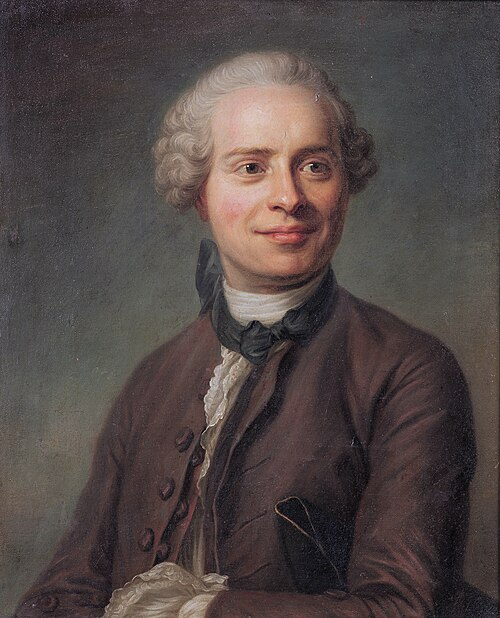
\includegraphics[width=0.30\textwidth]{Figures/dAlembert.png}
    \caption{Jean le Rond d'Alembert}
\end{figure}


% ============================================================
% LAGRANGE
% ============================================================
\newpage
\section*{\underline{\textbf{Joseph-Louis Lagrange (1736--1813)}}}

\textbf{Nationality:} Italian-French

\textbf{Generally known for:} Lagrange was a mathematician and physicist who made major contributions to analytical mechanics, calculus of variations, number theory, and celestial mechanics.

\textbf{Contribution to fluid mechanics:}

Lagrange developed mathematical methods for describing mechanics using generalized coordinates and energy principles. His work helped establish the distinction between following an individual particle and describing the entire velocity field.

In a Lagrangian description of a fluid, one follows an individual fluid particle:

\[
\frac{d\mathbf{x}}{dt}=\mathbf{u}(\mathbf{x},t).
\]

This approach remains fundamental to particle-based descriptions of fluid motion and is especially useful when following water parcels in oceanography. Lagrange's analytical mechanics also provided mathematical tools later used in fluid dynamics and geophysical fluid mechanics.

\begin{figure}[H]
    \centering
    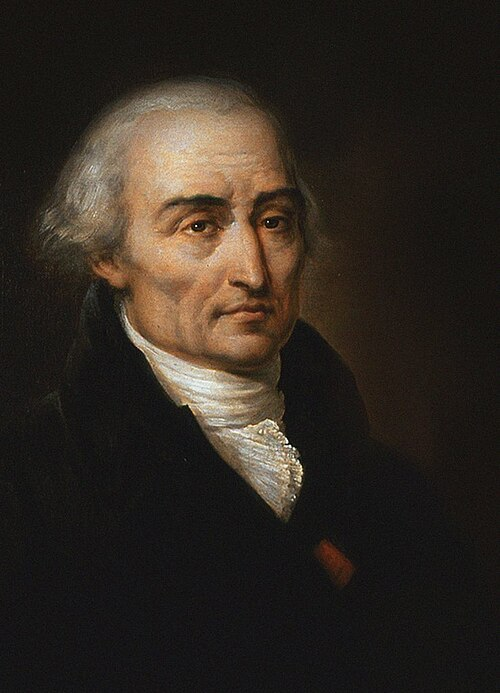
\includegraphics[width=0.30\textwidth]{Figures/Lagrange.png}
    \caption{Joseph-Louis Lagrange}
\end{figure}


% ============================================================
% LAPLACE
% ============================================================
\newpage
\section*{\underline{\textbf{Pierre-Simon Laplace (1749--1827)}}}

\textbf{Nationality:} French

\textbf{Generally known for:} Laplace was a mathematician, physicist, astronomer, and probability theorist. He made major contributions to celestial mechanics, probability, and mathematical physics.

\textbf{Contribution to fluid mechanics and atmospheric physics:}

Laplace investigated the propagation of sound in gases and corrected Newton's earlier treatment. The speed of sound in an ideal gas is

\[
c=\sqrt{\frac{\gamma p}{\rho}},
\]

where \(\gamma\) is the ratio of specific heats. The correction was important because compression and expansion during sound propagation occur rapidly enough to be approximately adiabatic rather than isothermal.

Laplace also developed mathematical methods involving potential functions, differential equations, and spherical geometry that later became fundamental in geophysical fluid dynamics and gravitational theory.

\begin{figure}[H]
    \centering
    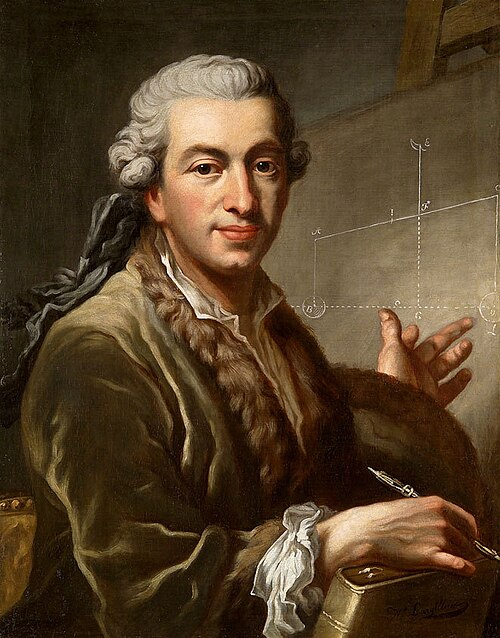
\includegraphics[width=0.30\textwidth]{Figures/Laplace.png}
    \caption{Pierre-Simon Laplace}
\end{figure}



% ============================================================
% NAVIER
% ============================================================
\newpage
\section*{\underline{\textbf{Claude-Louis Navier (1785--1836)}}}

\textbf{Nationality:} French

\textbf{Generally known for:} Navier was a mathematician, engineer, and physicist who worked on elasticity, bridges, and fluid mechanics.

\textbf{Contribution to fluid mechanics:}

Navier extended the equations of fluid motion to include internal friction. The resulting equation has the form

\[
\rho
\left(
\frac{\partial \mathbf{u}}{\partial t}
+
\mathbf{u}\cdot\nabla\mathbf{u}
\right)
=
-\nabla p
+
\mu\nabla^2\mathbf{u}
+
\rho\mathbf{g},
\]

for an incompressible Newtonian fluid with constant viscosity. The viscous term

\[
\mu\nabla^2\mathbf{u}
\]

represents the diffusion of momentum caused by molecular interactions. Navier's work was one of the steps leading toward the modern Navier--Stokes equations.

\begin{figure}[H]
    \centering
    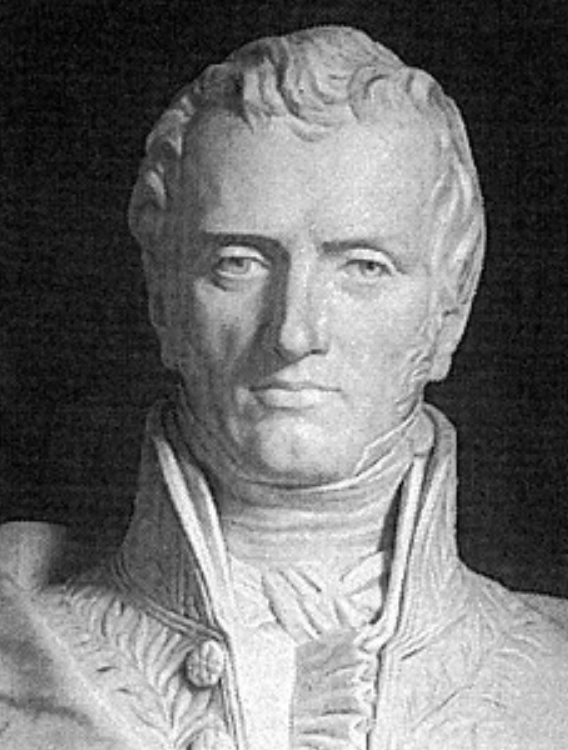
\includegraphics[width=0.30\textwidth]{Figures/Navier.png}
    \caption{Claude-Louis Navier}
\end{figure}


% ============================================================
% CORIOLIS
% ============================================================
\newpage
\section*{\underline{\textbf{Gaspard-Gustave de Coriolis (1792--1843)}}}

\textbf{Nationality:} French

\textbf{Generally known for:} Coriolis was a mathematician and engineer who worked on mechanics, machines, and rotating reference frames.

\textbf{Contribution to fluid mechanics and geophysics:}

Coriolis developed the mathematical description of the apparent forces that arise when motion is described in a rotating reference frame. For horizontal atmospheric and oceanic motion, the Coriolis parameter is

\[
f=2\Omega\sin\phi,
\]

where \(\Omega\) is Earth's angular rotation rate and \(\phi\) is latitude.

The Coriolis acceleration can be written

\[
\mathbf{a}_C=-2\boldsymbol{\Omega}\times\mathbf{u}.
\]

This term is essential for understanding large-scale atmospheric and oceanic circulation. It explains why winds and ocean currents are deflected relative to the direction of the pressure-gradient force. In the Northern Hemisphere the deflection is to the right of the motion, while in the Southern Hemisphere it is to the left.

\begin{figure}[H]
    \centering
    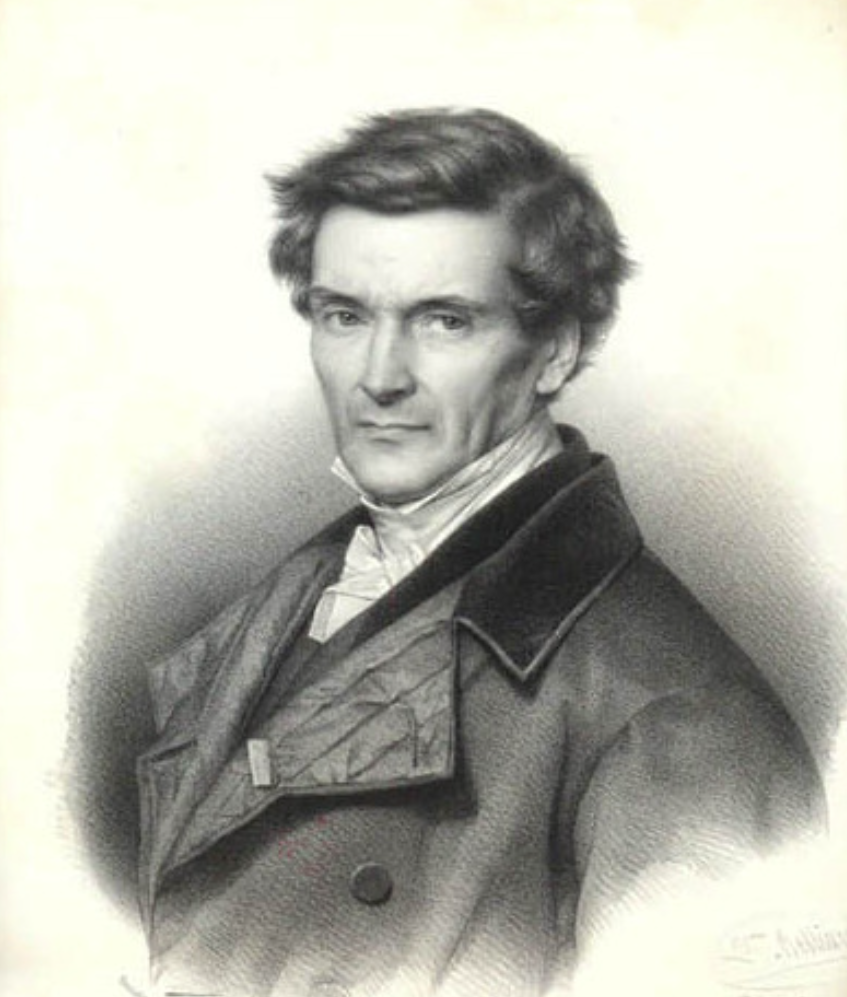
\includegraphics[width=0.30\textwidth]{Figures/Coriolis.png}
    \caption{Gaspard-Gustave de Coriolis}
\end{figure}




% ============================================================
% STOKES
% ============================================================
\newpage
\section*{\underline{\textbf{George Gabriel Stokes (1819--1903)}}}

\textbf{Nationality:} Irish-British

\textbf{Generally known for:} Stokes was a mathematician and physicist who worked on fluid mechanics, optics, mathematical physics, and spectroscopy.

\textbf{Contribution to fluid mechanics:}

Stokes studied the motion of very small particles through viscous fluids. For a small spherical particle moving slowly through a viscous fluid, the drag force is

\[
F_D=6\pi\mu r v \implies F_D\propto v.
\]

This is valid in the creeping-flow regime, where inertial effects are negligible. Stokes' law is used to determine settling velocities of particles, droplets, aerosols, and sediment grains.

Balancing gravitational settling against viscous drag gives the terminal settling speed of a small sphere:

\[
v_t=\frac{2r^2(\rho_p-\rho_f)g}{9\mu}.
\]

This result is highly important in sediment transport, atmospheric aerosols, ocean particles, and laboratory fluid mechanics.

\begin{figure}[H]
    \centering
    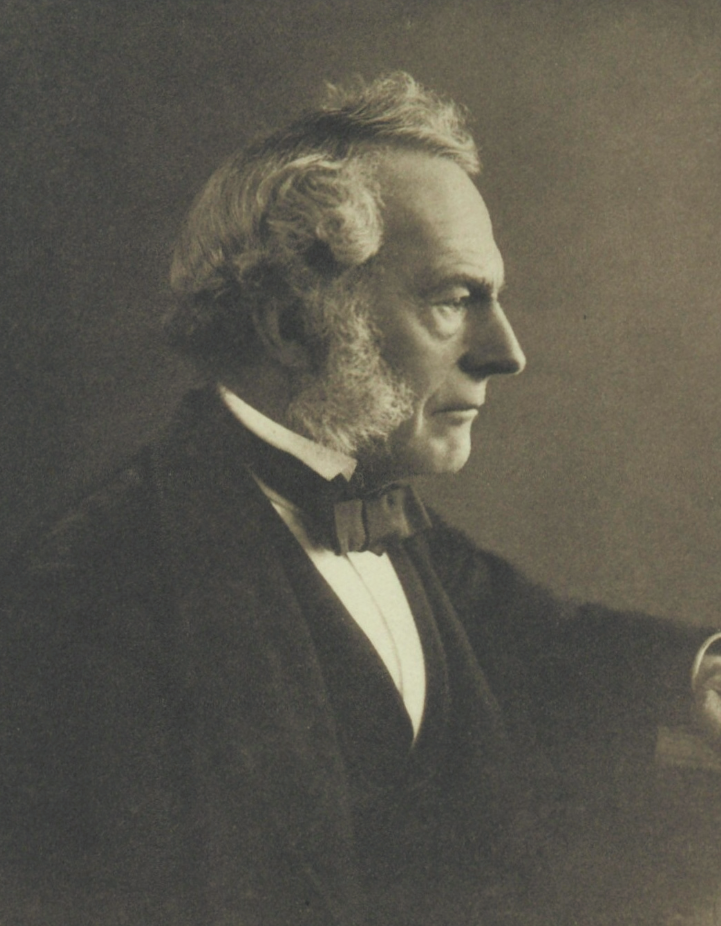
\includegraphics[width=0.30\textwidth]{Figures/Stokes.png}
    \caption{George Gabriel Stokes}
\end{figure}


% ============================================================
% CLAPEYRON
% ============================================================
\newpage
\section*{\underline{\textbf{Benoît Paul Émile Clapeyron (1799--1864)}}}

\textbf{Nationality:} French

\textbf{Generally known for:} Clapeyron was a physicist and engineer who worked on thermodynamics, steam engines, and railway engineering.

\textbf{Contribution to atmospheric and thermodynamic physics:}

Clapeyron developed a mathematical relationship describing phase changes. The general Clapeyron equation is

\[
\frac{dp}{dT}
=
\frac{L}{T\Delta v},
\]

where \(L\) is latent heat and \(\Delta v\) is the change in specific volume during the phase transition. For water vapour in the atmosphere, the relationship becomes approximately

\[
\frac{d\ln p_{\mathrm{sat}}}{dT}
\approx
\frac{L}{R_vT^2}.
\]

This relationship explains why the saturation vapour pressure of water increases rapidly with temperature. That fact is fundamental to cloud formation, atmospheric humidity, evaporation, condensation, and weather systems.

\begin{figure}[H]
    \centering
    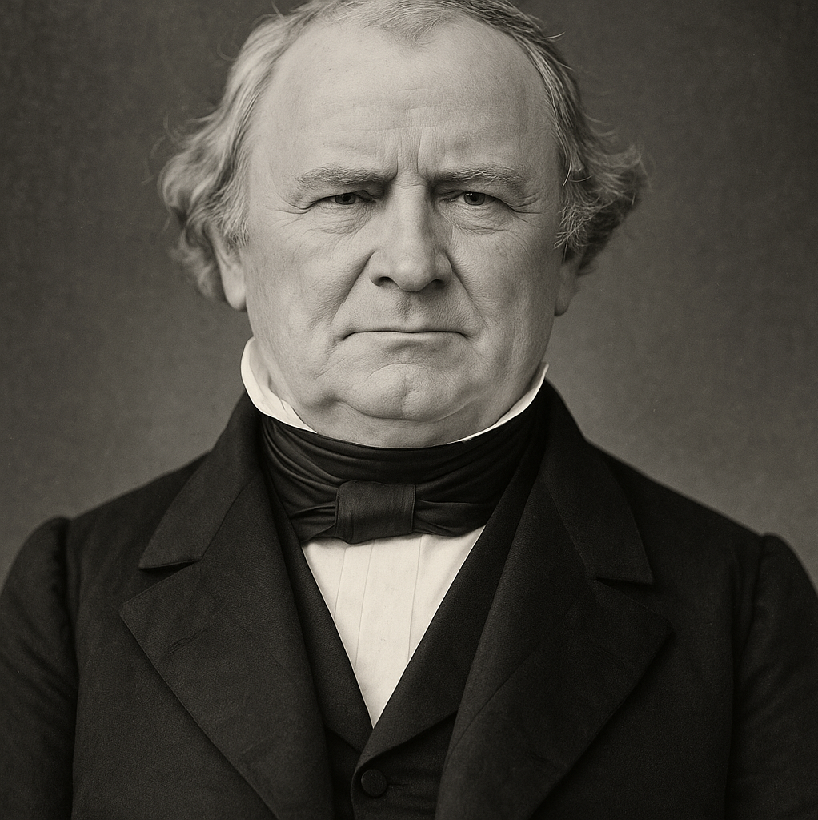
\includegraphics[width=0.30\textwidth]{Figures/Clapeyron.png}
    \caption{Benoît Paul Émile Clapeyron}
\end{figure}


% ============================================================
% CLAUSIUS
% ============================================================
\newpage
\section*{\underline{\textbf{Rudolf Julius Emanuel Clausius (1822--1888)}}}

\textbf{Nationality:} German

\textbf{Generally known for:} Clausius was a physicist and mathematician and one of the founders of thermodynamics.

\textbf{Contribution to atmospheric and fluid physics:}

Clausius introduced the modern concept of entropy and formulated one of the central mathematical statements of the second law of thermodynamics. For a reversible process,

\[
dS=\frac{\delta Q_{\mathrm{rev}}}{T}.
\]

Entropy became essential for describing irreversible processes and the thermodynamic behaviour of gases and fluids.

Clausius also developed the Clausius--Clapeyron equation, which describes how saturation vapour pressure changes with temperature:

\[
\frac{d\ln p_{\mathrm{sat}}}{dT}
\approx
\frac{L}{R_vT^2}.
\]

This relation is central to meteorology because atmospheric water vapour, condensation, evaporation, clouds, and precipitation are controlled by thermodynamic phase changes.

\begin{figure}[H]
    \centering
    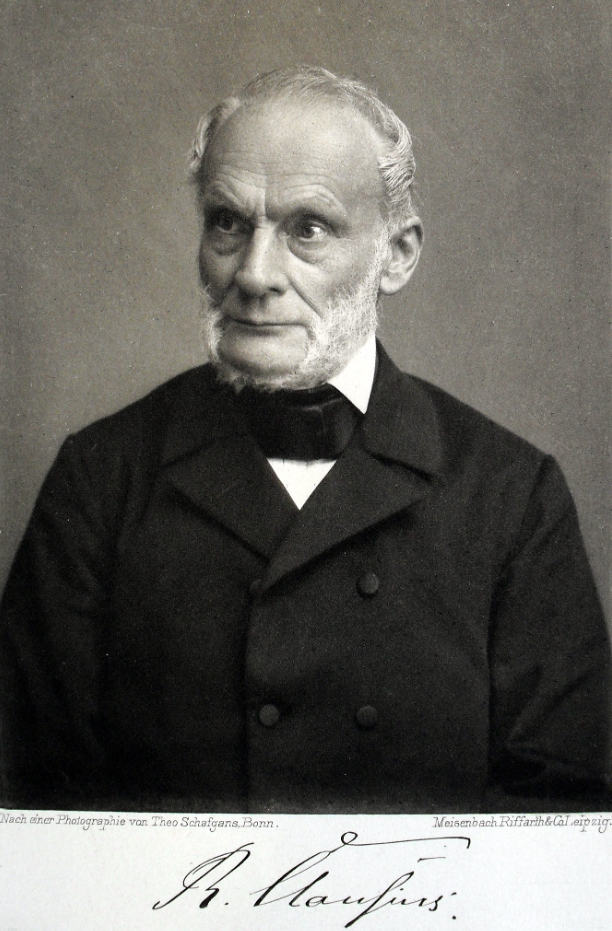
\includegraphics[width=0.30\textwidth]{Figures/Clausius.png}
    \caption{Rudolf Julius Emanuel Clausius}
\end{figure}


% ============================================================
% KELVIN
% ============================================================
\newpage
\section*{\underline{\textbf{William Thomson, Lord Kelvin (1824--1907)}}}

\textbf{Nationality:} Scottish-Irish

\textbf{Generally known for:} Kelvin was a physicist and mathematician who contributed to thermodynamics, electromagnetism, electrical engineering, heat theory, and geophysics.

\textbf{Contribution to fluid mechanics and oceanography:}

Kelvin made major contributions to the mathematical physics of fluids and rotating systems. He developed the circulation theorem now known as Kelvin's circulation theorem. For an inviscid, barotropic fluid subject to conservative body forces,

\[
\frac{D\Gamma}{Dt}=0,
\]

where

\[
\Gamma=\oint_C \mathbf{u}\cdot d\mathbf{l}
\]

is the circulation around a material closed curve. This result became a foundation for the study of vorticity and rotating flows.

Kelvin also studied waves and developed theory relevant to water waves and tidal motion. His work on rotating fluids contributed to the mathematical understanding of large-scale geophysical flows.

Kelvin's work also helped establish the absolute temperature scale and the thermodynamic framework needed to understand the atmosphere and ocean as energy-converting systems.

\begin{figure}[H]
    \centering
    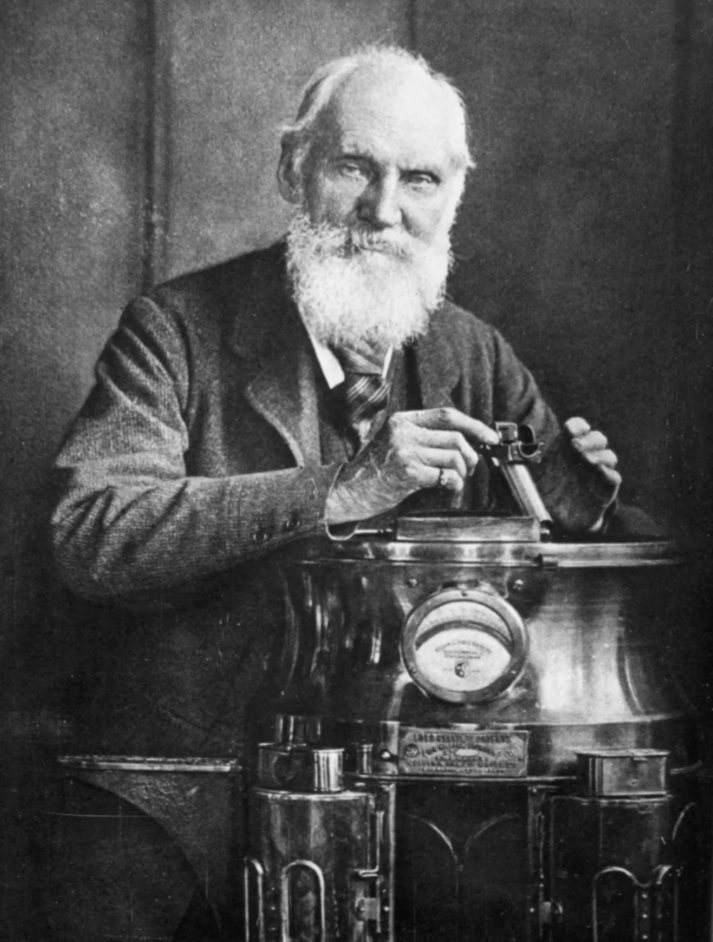
\includegraphics[width=0.30\textwidth]{Figures/Kelvin.png}
    \caption{William Thomson, Lord Kelvin}
\end{figure}


% ============================================================
% MAXWELL
% ============================================================
\newpage
\section*{\underline{\textbf{James Clerk Maxwell (1831--1879)}}}

\textbf{Nationality:} Scottish

\textbf{Generally known for:} Maxwell was a physicist and mathematician who formulated the theory of electromagnetism and made major contributions to kinetic theory and statistical physics.

\textbf{Contribution to fluid and gas physics:}

Maxwell developed a kinetic theory of gases in which macroscopic properties such as pressure and temperature emerge from the motion and collisions of microscopic molecules. He derived the Maxwell distribution of molecular velocities. The theory showed that gas viscosity is related to molecular motion and transport between neighbouring layers of gas.

Maxwell also introduced important ideas about molecular transport, including the mean free path of molecules. These ideas helped explain why quantities such as momentum, heat, and mass can be transported through a fluid by molecular motion. His work provided an important bridge between microscopic molecular physics and macroscopic fluid mechanics.

\begin{figure}[H]
    \centering
    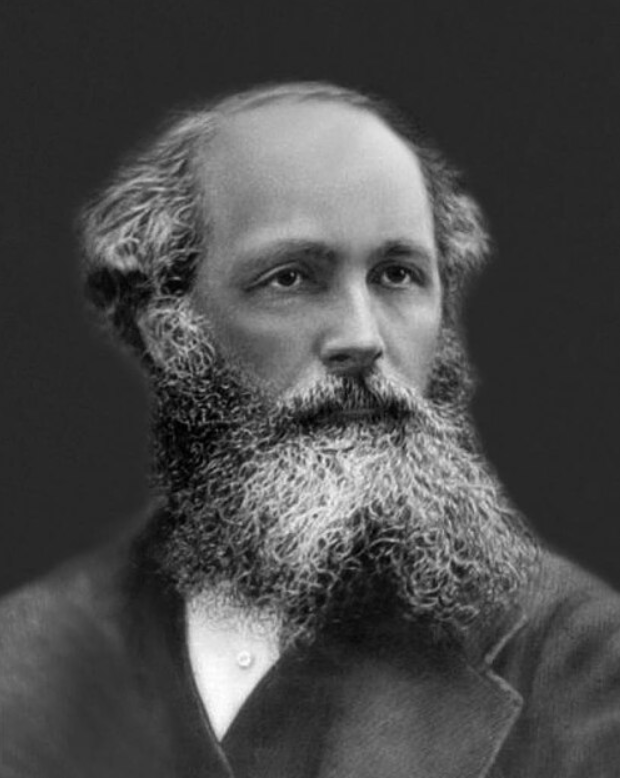
\includegraphics[width=0.30\textwidth]{Figures/Maxwell.png}
    \caption{James Clerk Maxwell}
\end{figure}


% ============================================================
% FERREL
% ============================================================
\newpage
\section*{\underline{\textbf{William Ferrel (1817--1891)}}}

\textbf{Nationality:} American

\textbf{Generally known for:} Ferrel was a meteorologist and professor who made major contributions to the understanding of atmospheric circulation.

\textbf{Contribution to meteorology:}

Ferrel recognized that large-scale atmospheric motion is strongly controlled by Earth's rotation and by the conservation of angular momentum. He developed a theory of the midlatitude circulation and showed why the winds in the middle latitudes cannot be understood simply as air moving directly from the equator toward the poles. In the Northern Hemisphere, moving air experiences a Coriolis deflection to the right, producing the prevailing westerlies of the midlatitudes. In the Southern Hemisphere, the corresponding deflection is to the left.

Ferrel's work helped establish the three-cell picture of global atmospheric circulation that is now associated with the Hadley, Ferrel, and polar cells.

\begin{figure}[H]
    \centering
    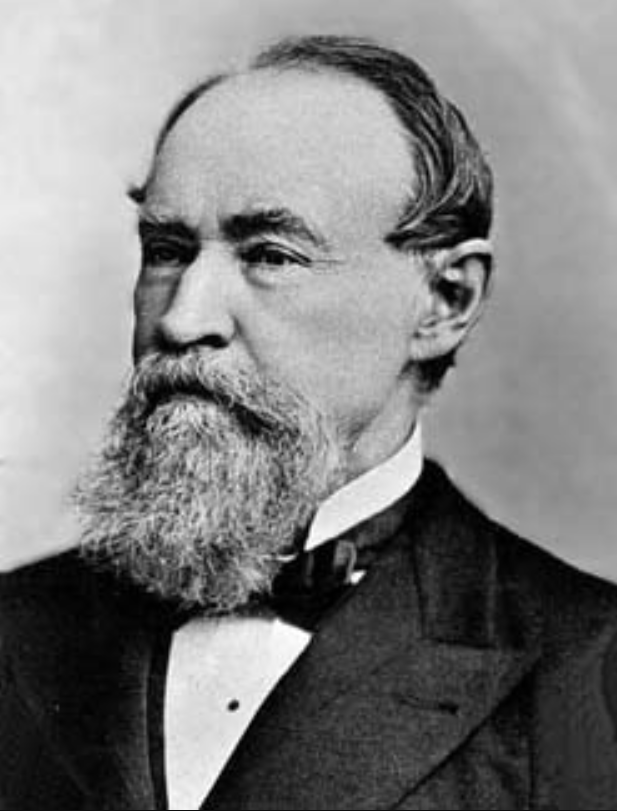
\includegraphics[width=0.30\textwidth]{Figures/Ferrel.png}
    \caption{William Ferrel}
\end{figure}


% ============================================================
% BOUSSINESQ
% ============================================================
\newpage
\section*{\underline{\textbf{Joseph Valentin Boussinesq (1842--1929)}}}

\textbf{Nationality:} French

\textbf{Generally known for:} Boussinesq was a mathematician and physicist who worked on fluid mechanics, elasticity, heat transfer, and applied mathematics.

\textbf{Contribution to fluid mechanics and geophysical flows:}

Boussinesq developed the approximation that bears his name. In many flows, density variations are small and can be ignored almost everywhere except where gravity converts those density differences into buoyancy. Thus, $\rho\approx\rho_0$ in most terms of the momentum equation, while density variations are retained in the buoyancy term. This approximation is fundamental to convection, atmospheric flows, ocean circulation, and laboratory experiments involving temperature-driven motion.

Boussinesq also developed an important approach to turbulent transport in which turbulent fluxes are related to mean gradients. A simple gradient-diffusion representation is

\[
F_\phi=-K\frac{d\phi}{dz}.
\]

For turbulent momentum transport this leads schematically to

\[
\tau_t\approx\rho K_m\frac{dU}{dz},
\]

with the precise sign depending on the coordinate and stress convention. These ideas became foundational for modelling turbulent geophysical flows.

\begin{figure}[H]
    \centering
    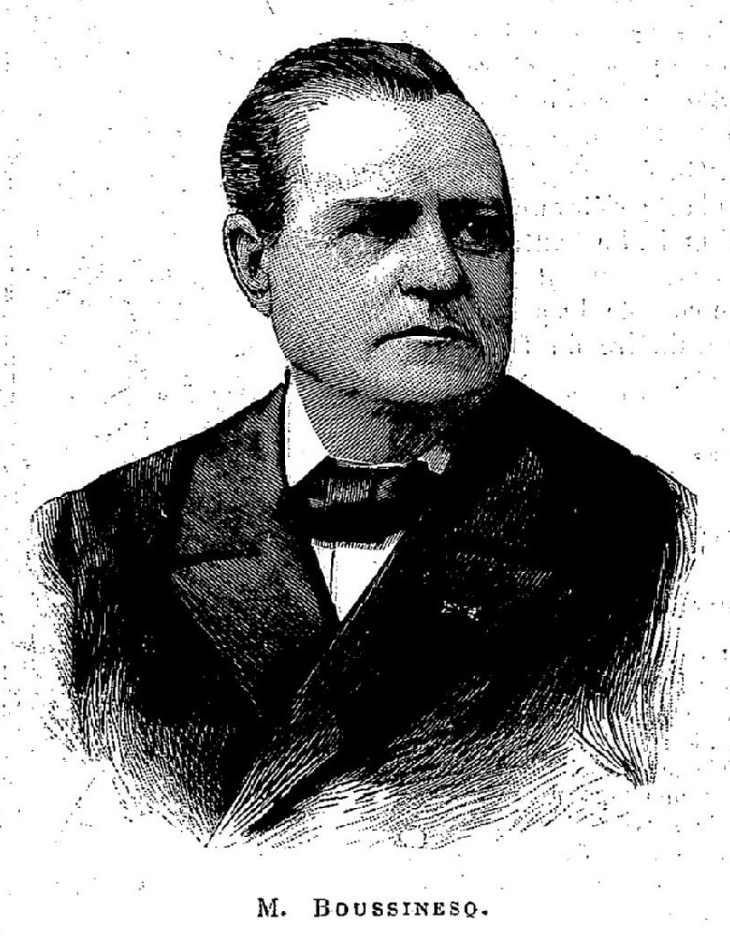
\includegraphics[width=0.30\textwidth]{Figures/Boussinesq.png}
    \caption{Joseph Valentin Boussinesq}
\end{figure}


% ============================================================
% RAYLEIGH
% ============================================================
\newpage
\section*{\underline{\textbf{John William Strutt, 3rd Baron Rayleigh (1842--1919)}}}

\textbf{Nationality:} English

\textbf{Generally known for:} Rayleigh was a physicist and mathematician who worked on acoustics, optics, wave theory, electromagnetism, and fluid mechanics.

\textbf{Contribution to fluid mechanics:}

Rayleigh studied fluid instability and convection. One of the key dimensionless numbers associated with buoyancy-driven flow is the Rayleigh number:

\[
Ra=
\frac{g\alpha\Delta T L^3}{\nu\kappa},
\]

where \(g\) is gravitational acceleration, \(\alpha\) is thermal expansion coefficient, \(\Delta T\) is the temperature difference, \(L\) is the characteristic length, \(\nu\) is kinematic viscosity, and \(\kappa\) is thermal diffusivity. Large \(Ra\) means buoyancy is strong compared with viscous and thermal-diffusion effects, making convection more likely.

Rayleigh also investigated waves and instabilities, helping establish the mathematical treatment of instability that became central to modern fluid dynamics.

\begin{figure}[H]
    \centering
    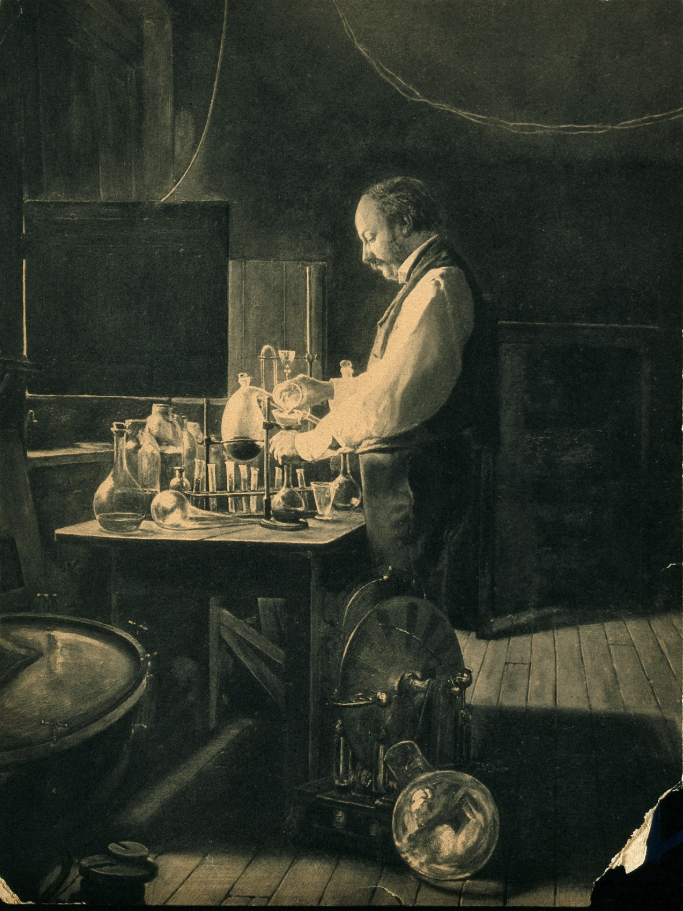
\includegraphics[width=0.30\textwidth]{Figures/Rayleigh.png}
    \caption{John William Strutt, 3rd Baron Rayleigh}
\end{figure}


% ============================================================
% REYNOLDS
% ============================================================
\newpage
\section*{\underline{\textbf{Osborne Reynolds (1842--1912)}}}

\textbf{Nationality:} English

\textbf{Generally known for:} Reynolds was an engineer and physicist who worked on hydraulics, heat transfer, and fluid mechanics.

\textbf{Contribution to fluid mechanics:}

Reynolds experimentally investigated the transition between smooth laminar flow and irregular turbulent flow. In his famous pipe-flow experiments, he injected dye into flowing water. At low flow speeds, the dye remained in a narrow, coherent streak. At higher speeds, the dye rapidly spread across the pipe as the flow became turbulent. He identified the dimensionless Reynolds number

\[
Re=\frac{\rho UL}{\mu}
=
\frac{UL}{\nu}.
\]

It compares inertial effects with viscous effects. Small \(Re\) generally corresponds to viscous-dominated flow, while large \(Re\) indicates that inertial effects are more important and turbulence becomes possible.

Reynolds also introduced the decomposition

\[
u=U+u',
\]

where \(U\) is the mean velocity and \(u'\) is the fluctuating component. This led to the Reynolds-averaged Navier--Stokes equations and the concept of turbulent stresses.

\begin{figure}[H]
    \centering
    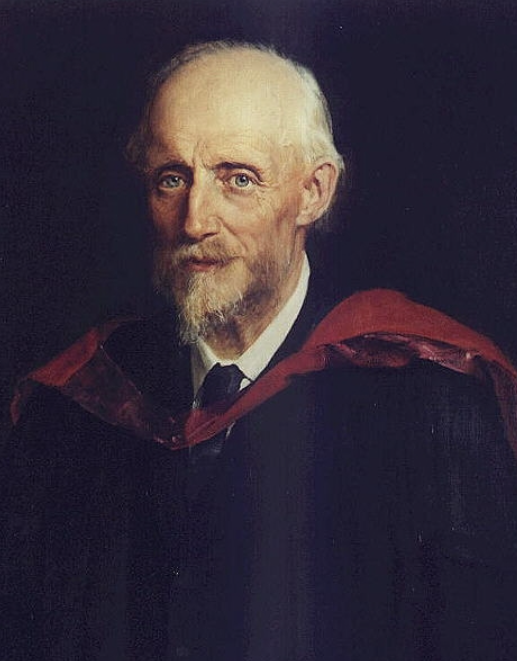
\includegraphics[width=0.30\textwidth]{Figures/Reynolds.png}
    \caption{Osborne Reynolds}
\end{figure}


% ============================================================
% MAURY
% ============================================================
\newpage
\section*{\underline{\textbf{Matthew Fontaine Maury (1806--1873)}}}

\textbf{Nationality:} American

\textbf{Generally known for:} Maury was a naval officer, hydrographer, oceanographer, and pioneer of scientific navigation.

\textbf{Contribution to physical oceanography:}

Maury collected enormous quantities of observations from ships travelling across the oceans. He organized ship logs containing measurements of winds, currents, temperatures, and sailing conditions and converted them into systematic charts. These charts allowed navigators to identify recurring wind patterns and ocean currents and choose faster sailing routes.

Maury's work was important because it transformed scattered observations into a large-scale observational description of the oceans. His efforts also helped establish international cooperation in collecting oceanographic observations.

\begin{figure}[H]
    \centering
    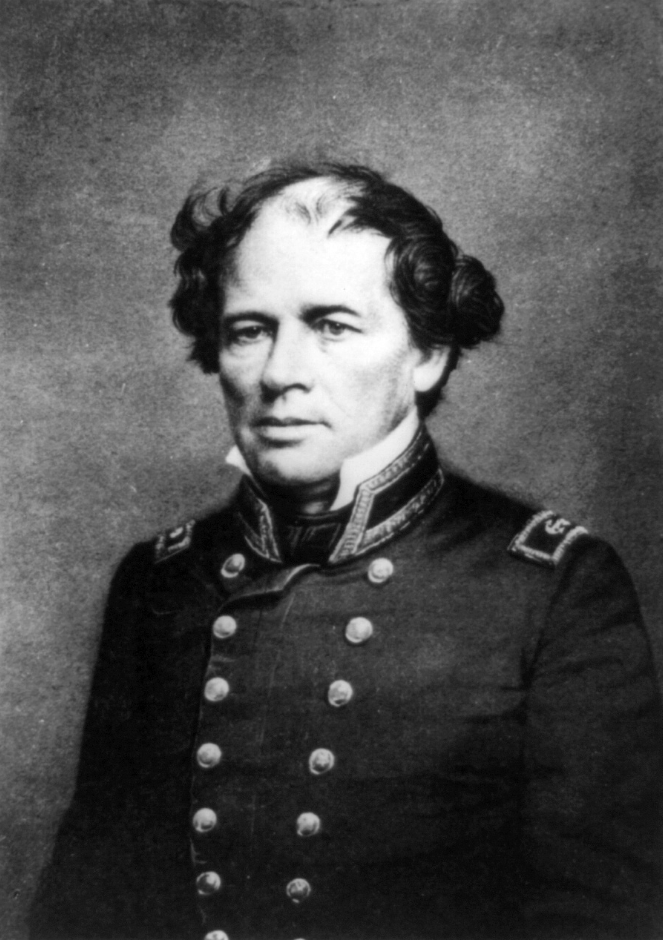
\includegraphics[width=0.30\textwidth]{Figures/Maury.png}
    \caption{Matthew Fontaine Maury}
\end{figure}


% ============================================================
% CHARLES WYVILLE THOMSON
% ============================================================
\newpage
\section*{\underline{\textbf{Charles Wyville Thomson (1830--1882)}}}

\textbf{Nationality:} Scottish

\textbf{Generally known for:} Thomson was a marine biologist and naturalist who became a leading figure in nineteenth-century deep-sea exploration.

\textbf{Contribution to physical oceanography:}

Thomson was the scientific leader of the \textit{Challenger} expedition from 1872 to 1876. The expedition travelled around the world's oceans and collected systematic measurements of depth, temperature, seawater properties, sediments, and marine life. The expedition demonstrated that the deep ocean was not biologically dead and that ocean conditions varied systematically with depth and location.

Its measurements provided one of the first global observational datasets for physical and biological oceanography.

\begin{figure}[H]
    \centering
    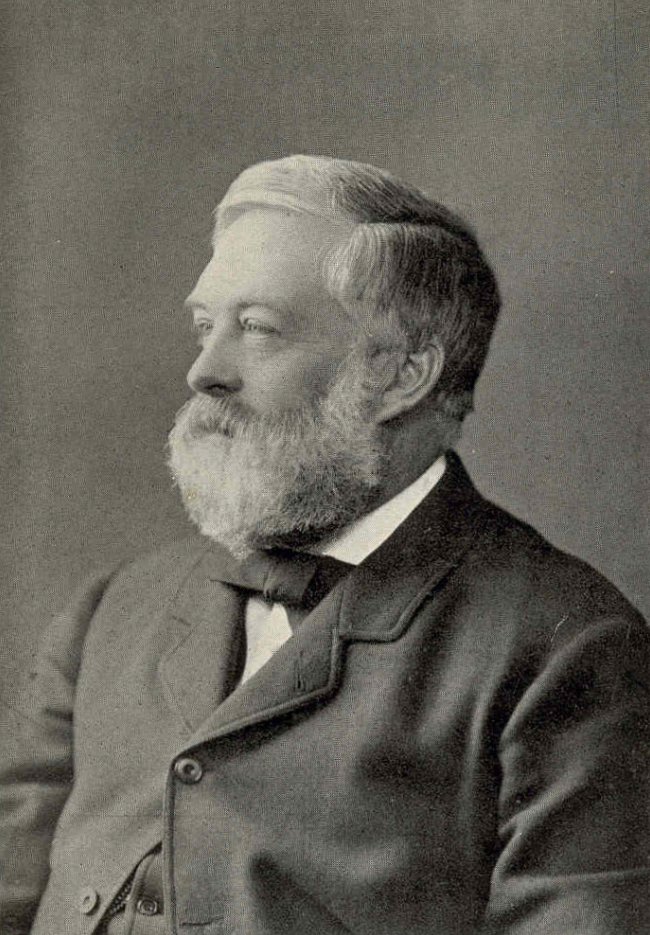
\includegraphics[width=0.30\textwidth]{Figures/Thomson.png}
    \caption{Charles Wyville Thomson}
\end{figure}


% ============================================================
% JOHN MURRAY
% ============================================================
\newpage
\section*{\underline{\textbf{Sir John Murray (1841--1914)}}}

\textbf{Nationality:} Scottish

\textbf{Generally known for:} Murray was a marine scientist and one of the founders of modern oceanography.

\textbf{Contribution to physical oceanography:}

Murray participated in the \textit{Challenger} expedition and later analyzed enormous quantities of oceanographic data. He investigated ocean depth, marine sediments, temperature distributions, ocean circulation, and the formation of deep-sea deposits.

He recognized that the oceans should be studied as interconnected physical systems rather than as isolated collections of biological organisms. Murray's work helped establish physical oceanography as a distinct scientific discipline.

\begin{figure}[H]
    \centering
    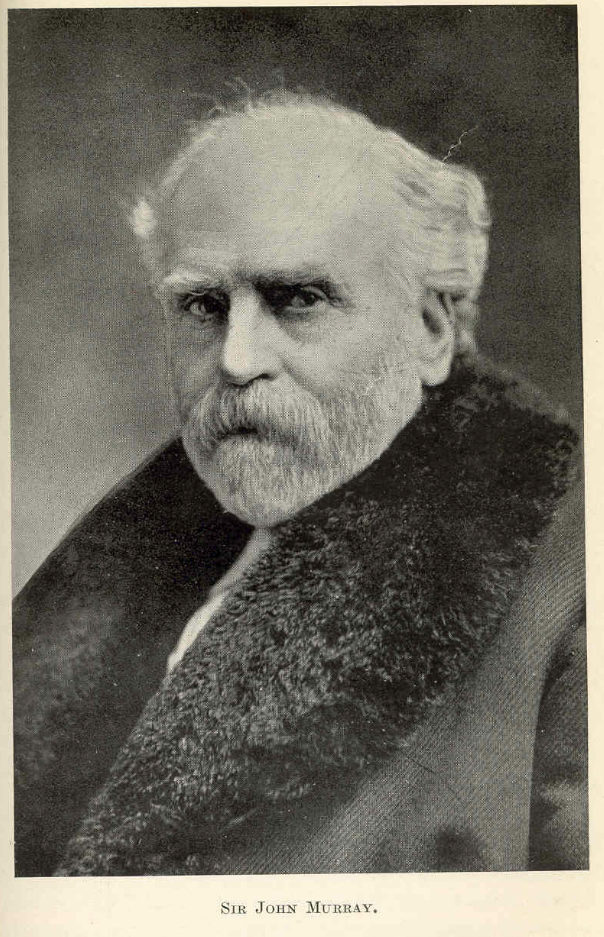
\includegraphics[width=0.30\textwidth]{Figures/Murray.png}
    \caption{Sir John Murray}
\end{figure}


% ============================================================
% NANSEN
% ============================================================
\newpage
\section*{\underline{\textbf{Fridtjof Nansen (1861--1930)}}}

\textbf{Nationality:} Norwegian

\textbf{Generally known for:} Nansen was an explorer, scientist, diplomat, and humanitarian. He was awarded the Nobel Peace Prize in 1922.

\textbf{Contribution to physical oceanography:}

Nansen led the \textit{Fram} expedition into the Arctic Ocean. The \textit{Fram} was deliberately allowed to become frozen into the sea ice. Instead of remaining stationary, the ship drifted with the moving ice.

Nansen noticed that the direction of ice drift was not simply the same as the wind. The drift was systematically deflected. This observation became one of the clues leading to the later mathematical explanation of wind-driven ocean currents by Vagn Walfrid Ekman.

Nansen also collected measurements of temperature and salinity from the Arctic Ocean and demonstrated the existence of distinct water masses at different depths.

\begin{figure}[H]
    \centering
    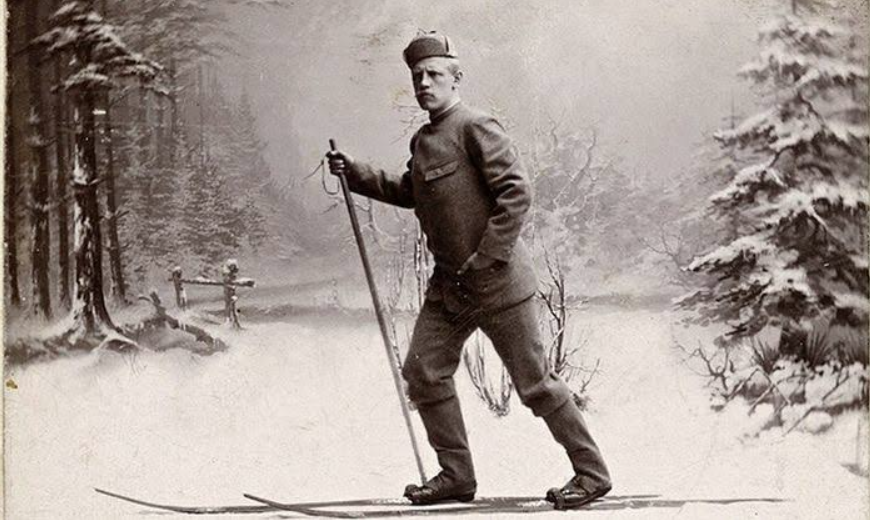
\includegraphics[width=0.55\textwidth]{Figures/Nansen.png}
    \caption{Fridtjof Nansen}
\end{figure}


% ============================================================
% BJERKNES
% ============================================================
\newpage
\section*{\underline{\textbf{Vilhelm Frimann Koren Bjerknes (1862--1951)}}}

\textbf{Nationality:} Norwegian

\textbf{Generally known for:} Bjerknes was a physicist and meteorologist who established much of the mathematical foundation of modern weather prediction.

\textbf{Contribution to meteorology:}

Bjerknes recognized that weather prediction could be treated as an initial-value problem in fluid dynamics and thermodynamics. In principle, if the atmospheric variables could be measured sufficiently accurately at one time, their future evolution could be calculated from the governing physical laws. These variables include:

\begin{itemize}
\item $\vec{u}$ -- velocity field
\item $p$ -- atmospheric pressure
\item $T$ -- temperature
\item $\rho$ -- air density
\item $q$ -- humidity or water-vapour content
\end{itemize}

These variables are linked through the equations of fluid motion, conservation of mass, thermodynamics, the equation of state, and moisture processes. Bjerknes therefore helped transform meteorology from a largely descriptive science into a quantitative physical science.

Bjerknes also founded the Bergen school of meteorology, where these ideas were developed further through the study of atmospheric fronts, cyclones, air masses, and weather evolution. His work provided an important foundation for modern weather forecasting and atmospheric dynamics.


\begin{figure}[H]
    \centering
    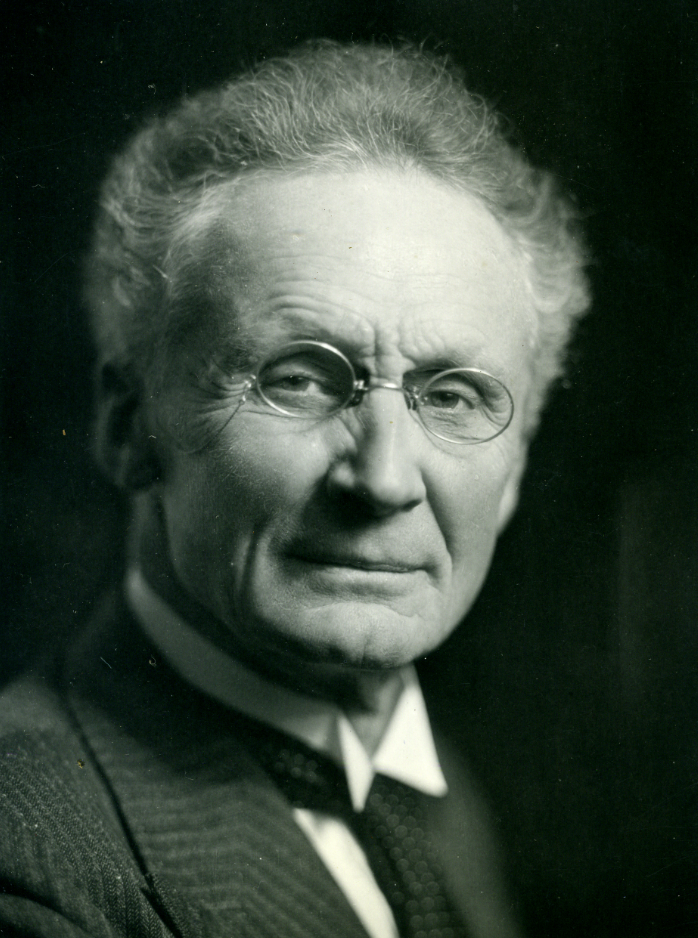
\includegraphics[width=0.30\textwidth]{Figures/Bjerknes.png}
    \caption{Vilhelm Frimann Koren Bjerknes}
\end{figure}
% ============================================================
% David Brunt
% ============================================================
\newpage
\section*{\underline{\textbf{David Brunt (1886--1965)}}}

\textbf{Nationality:} British

\textbf{Generally known for:} David Brunt was a British meteorologist and mathematician known for his work on atmospheric stability, stratification, and dynamic meteorology.

\textbf{Contribution to fluid mechanics:}

Brunt studied the vertical motion of air parcels in a stratified atmosphere. He showed that when an air parcel is displaced vertically, differences between its density and the surrounding air can produce a restoring force. For stable stratification, the parcel oscillates about its equilibrium position according to

$$
\frac{d^2\xi}{dt^2}+N^2\xi=0,
$$

where \(N\) is the buoyancy frequency. The quantity \(N\) is now known as the {Brunt--Väisälä frequency},

$$
N^2=\frac{g}{\theta}\frac{d\theta}{dz}.
$$

A positive \(N^2\) indicates stable stratification, while the magnitude of \(N\) measures the strength of the restoring effect. This concept became fundamental in the study of atmospheric and oceanic stratification, internal waves, convection, and vertical mixing.

In 1926, Brunt published \textit{Periodicities in European Weather}, in which he investigated recurring patterns in European weather and their possible physical causes, contributing to the early development of statistical and dynamical approaches to weather prediction.

\begin{figure}[H]
    \centering
    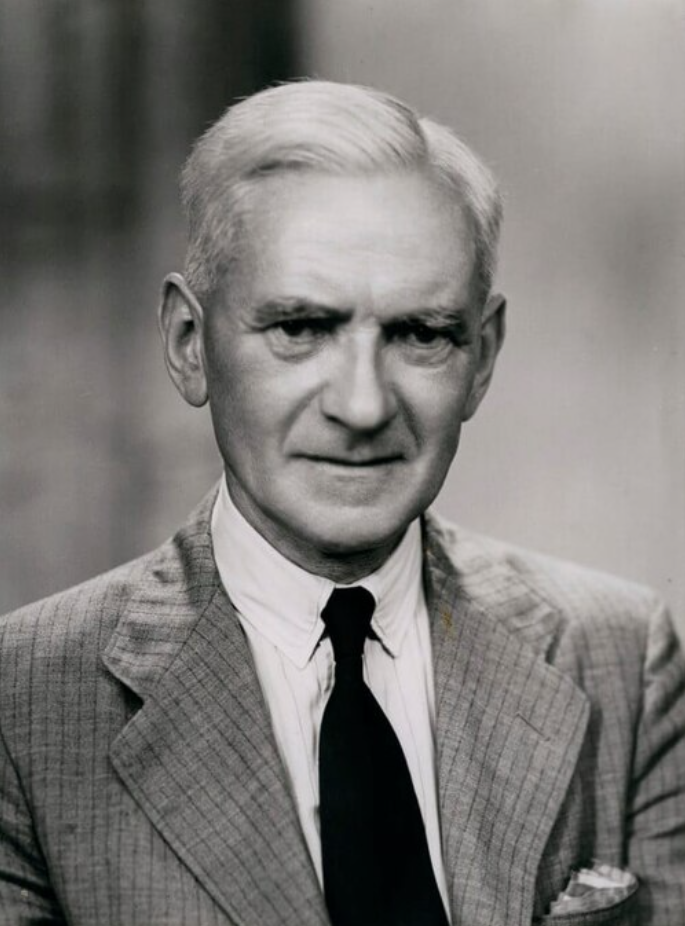
\includegraphics[width=0.30\textwidth]{Figures/Brunt.png}
    \caption{David Brunt}
\end{figure}

% ============================================================
% PRANDTL
% ============================================================
\newpage
\section*{\underline{\textbf{Ludwig Prandtl (1875--1953)}}}

\textbf{Nationality:} German

\textbf{Generally known for:} Prandtl was a physicist and engineer and is often considered one of the founders of modern fluid mechanics. His work connected mathematical fluid mechanics with practical problems in aerodynamics and engineering.

\textbf{Contribution to fluid mechanics:}

Prandtl developed boundary-layer theory. For a real viscous fluid flowing over a solid surface, the no-slip condition requires $ u=0 $ at the wall. However, outside a relatively thin region near the surface, viscosity may have a much smaller direct influence on the flow. Prandtl recognized that the flow can therefore be separated conceptually into an outer region where inviscid approximations may work well and a thin boundary layer where viscosity is crucial. This explained how real fluids can experience drag even though ideal-fluid theory can predict zero drag, resolving the physical difficulty highlighted by d'Alembert's paradox.

Prandtl also developed the mixing-length hypothesis to describe turbulent momentum transport. He proposed that turbulent eddies move fluid parcels over a characteristic distance, \(l_m\), before their momentum is significantly changed by the surrounding fluid. This led to a simple estimate for the turbulent shear stress,

\[
\tau_t \approx \rho l_m^2
\left|\frac{dU}{dz}\right|
\frac{dU}{dz},
\]

which can be interpreted as an additional, turbulence-generated momentum transport analogous to the effect of molecular viscosity. 

Prandtl's boundary-layer theory and mixing-length concept became fundamental to aircraft aerodynamics, pipe flow, atmospheric surface layers and ocean currents.

\begin{figure}[H]
    \centering
    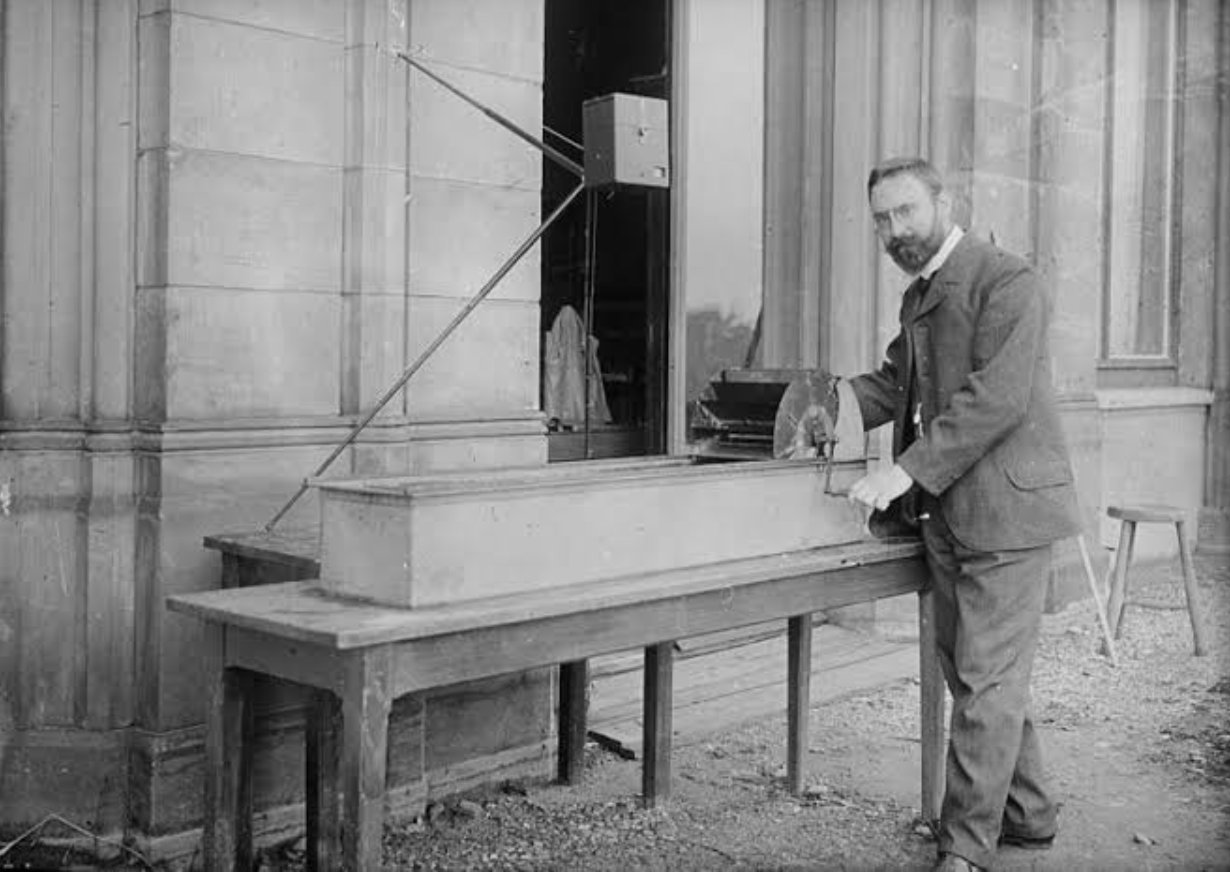
\includegraphics[width=0.45\textwidth]{Figures/Prandtl.png}
    \caption{Ludwig Prandtl is shown next to a water channel}
\end{figure}


% ============================================================
% EKMAN
% ============================================================
\newpage
\section*{\underline{\textbf{Vagn Walfrid Ekman (1874--1954)}}}

\textbf{Nationality:} Swedish

\textbf{Generally known for:} Ekman was a Swedish oceanographer and physical oceanographer.

\textbf{Contribution to physical oceanography:}

Ekman developed the theory explaining how wind stress produces ocean currents in a rotating Earth system. Nansen's Arctic observations showed that ice drift was systematically deflected relative to the wind. Ekman developed a mathematical explanation using a balance between wind stress, frictional momentum transfer, and the Coriolis force.

The result is the Ekman spiral: velocity changes both magnitude and direction with depth. In an idealized steady ocean surface layer, the vertically integrated transport as

\[
\mathbf{M_E}=\frac{1}{\rho f}\hat{z}\times \vec{\tau},
\]

where \(\tau\) is wind stress, \(\rho\) is seawater density, and \(f\) is the Coriolis parameter. The transport is directed approximately \(90^\circ\) to the wind stress, with the direction depending on hemisphere and sign convention. Ekman's theory was a major step in explaining how atmospheric winds produce large-scale ocean circulation.

\begin{figure}[H]
    \centering
    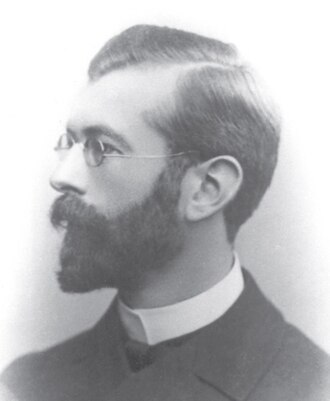
\includegraphics[width=0.30\textwidth]{Figures/Ekman.png}
    \caption{Vagn Walfrid Ekman}
\end{figure}


% ============================================================
% RICHARDSON
% ============================================================
\newpage
\section*{\underline{\textbf{Lewis Fry Richardson (1881--1953)}}}

\textbf{Nationality:} English

\textbf{Generally known for:} Richardson was a mathematician, physicist, meteorologist, psychologist, and pacifist. He also made important contributions to the mathematical study of conflict and statistics.

\textbf{Contribution to numerical weather prediction:}

Richardson was one of the first people to seriously attempt numerical weather prediction. He recognized that atmospheric evolution could be represented by differential equations and that these equations could be approximated numerically on a grid. He attempted to calculate the future atmospheric pressure field from observations using finite-difference approximations. His famous calculation took enormous effort and produced an unrealistic result because the initial data and numerical procedure were not sufficiently stable. The failure nevertheless demonstrated something fundamental: weather prediction requires both a physical model and an enormous amount of computation.

Richardson imagined a future ``forecast factory'' in which large numbers of people would perform calculations simultaneously. Modern numerical weather prediction eventually realized the computational idea he had envisioned.

\begin{figure}[H]
    \centering
    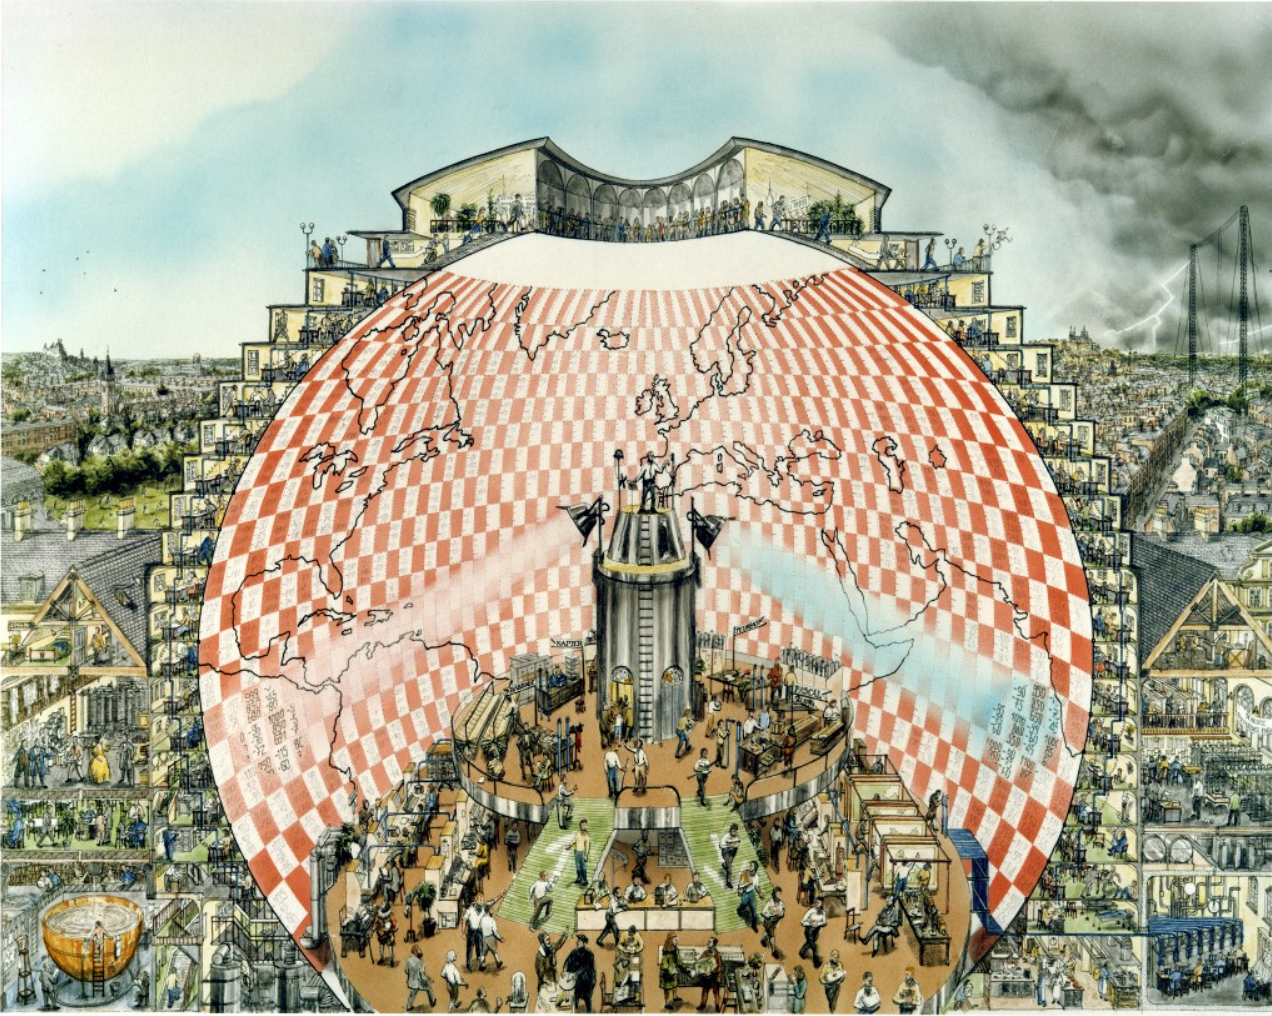
\includegraphics[width=0.50\textwidth]{Figures/Richardson.png}
    \caption{W\textit{eather Forecasting Factory} by Stephen Conlin, based on the description by L.F. Richardson}
\end{figure}

% ============================================================
% Gilbert Walker 
% ============================================================

\newpage

\section*{\underline{\textbf{Gilbert Walker (1868--1958)}}}

\textbf{Nationality:} British

\textbf{Generally known for:} Gilbert Walker was a British mathematician and meteorologist known for identifying large-scale patterns of atmospheric pressure and circulation.

\textbf{Contribution to fluid mechanics:}

Walker studied relationships between atmospheric pressure, winds, and rainfall using long-term weather observations. In the 1920s, he identified the Southern Oscillation, a large-scale variation in atmospheric pressure between the western and eastern tropical Pacific. This oscillation is closely linked to El Niño, and the combined ocean--atmosphere phenomenon is now known as ENSO(El Niño--Southern Oscillation). Walker also identified important pressure relationships associated with the North Atlantic Oscillation (NAO), describing how variations in the pressure difference between the Azores region and Iceland are related to changes in European weather and atmospheric circulation.

Walker's work demonstrated that weather patterns in widely separated regions can be statistically connected, providing an important foundation for the modern study of large-scale atmospheric circulation and climate variability.

\begin{figure}[H]
    \centering
    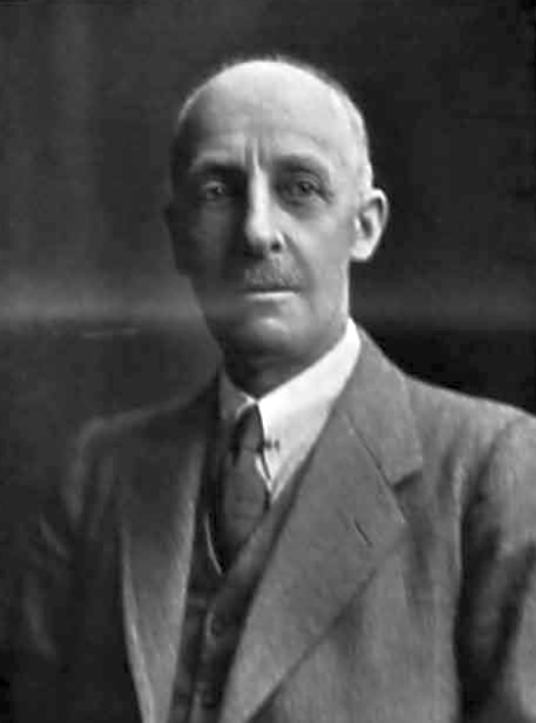
\includegraphics[width=0.30\textwidth]{Figures/Walker.png}
    \caption{Gilbert Walker}
\end{figure}




% ============================================================
% VON KARMAN
% ============================================================
\newpage
\section*{\underline{\textbf{Theodore von Kármán (1881--1963)}}}

\textbf{Nationality:} Hungarian-American

\textbf{Generally known for:} Von Kármán was a mathematician, physicist, aerospace engineer, and pioneer of aerodynamics and rocketry.

\textbf{Contribution to fluid mechanics:}

Von Kármán studied vortex shedding behind bluff bodies. When a fluid flows past a cylindrical obstacle, vortices can detach alternately from opposite sides of the body. This produces a repeating pattern called a von Kármán vortex street. Von Kármán's work helped establish the importance of coherent vortices in turbulent and separated flows.

Von Kármán also contributed to the theory of turbulent boundary layers and the logarithmic velocity profile. In the near-surface region of a turbulent flow, the mean velocity can be approximated by

\[
U(z)=\frac{u_*}{\kappa}\ln\left(\frac{z}{z_0}\right),
\]

where $u_*$ is the friction velocity, $z_0$ is the roughness length, and $\kappa\approx0.4$ is the von Kármán constant. This logarithmic wind law became fundamental for describing velocity profiles in the atmospheric surface layer and turbulent flows near solid boundaries.

\begin{figure}[H]
    \centering
    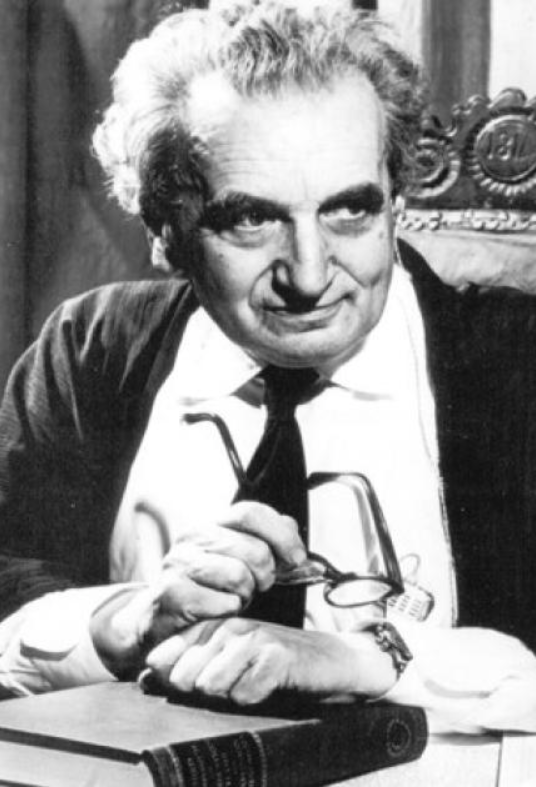
\includegraphics[width=0.30\textwidth]{Figures/Karman.png}
    \caption{Theodore von Kármán}
\end{figure}


% ============================================================
% GEOFFREY TAYLOR
% ============================================================
\newpage
\section*{\underline{\textbf{Geoffrey Ingram Taylor (1886--1975)}}}

\textbf{Nationality:} English

\textbf{Generally known for:} Taylor was a mathematician and physicist who worked on fluid mechanics, turbulence, elasticity, atmospheric physics, and the mechanics of explosions.

\textbf{Contribution to fluid mechanics:}

Taylor made fundamental contributions to turbulence and statistical fluid mechanics. Instead of treating turbulence as completely random noise, he studied statistical correlations between velocity fluctuations at different locations and times. He introduced concepts such as the Taylor microscale and developed theories describing turbulent diffusion and mixing. Taylor also investigated turbulent transport using dimensional and statistical arguments.

His work helped establish the modern idea that turbulence can be described through statistical quantities such as correlations, spectra, and characteristic length scales rather than by tracking every individual turbulent eddy.

\begin{figure}[H]
    \centering
    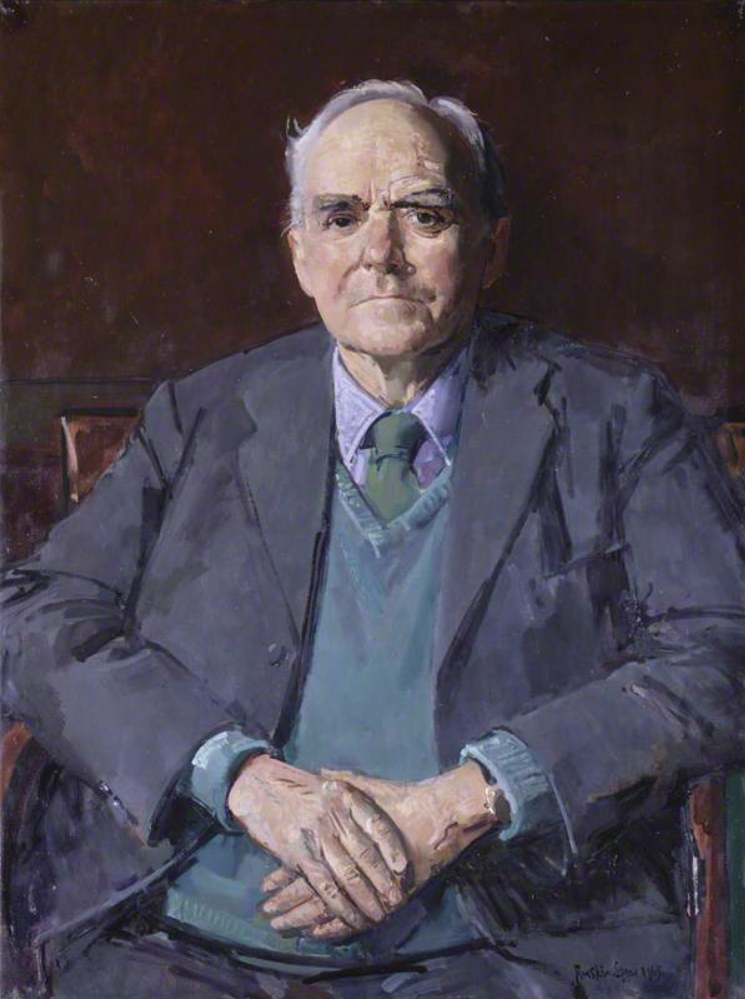
\includegraphics[width=0.30\textwidth]{Figures/Taylor.png}
    \caption{Geoffrey Ingram Taylor}
\end{figure}


% ============================================================
% SVERDRUP
% ============================================================
\newpage
\section*{\underline{\textbf{Harald Ulrik Sverdrup (1888--1957)}}}

\textbf{Nationality:} Norwegian

\textbf{Generally known for:} Sverdrup was a Norwegian oceanographer and polar scientist who worked on Arctic and global ocean circulation.

\textbf{Contribution to physical oceanography:}

Sverdrup developed a theory connecting wind-stress patterns over the ocean to large-scale interior ocean circulation. In a simplified form, the Sverdrup balance can be written

\[
\beta M=
\frac{\nabla\times\boldsymbol{\tau}}{\rho_0},
\]

where

\[
\beta=\frac{df}{dy},
\]

\(M\) is the vertically integrated meridional transport, \(\boldsymbol{\tau}\) is wind stress, and \(\rho_0\) is a reference seawater density. The equation shows that the curl of the wind stress can generate large-scale ocean transport.

Sverdrup's theory became one of the foundations for understanding subtropical gyres and the wind-driven circulation of the world's oceans.

\begin{figure}[H]
    \centering
    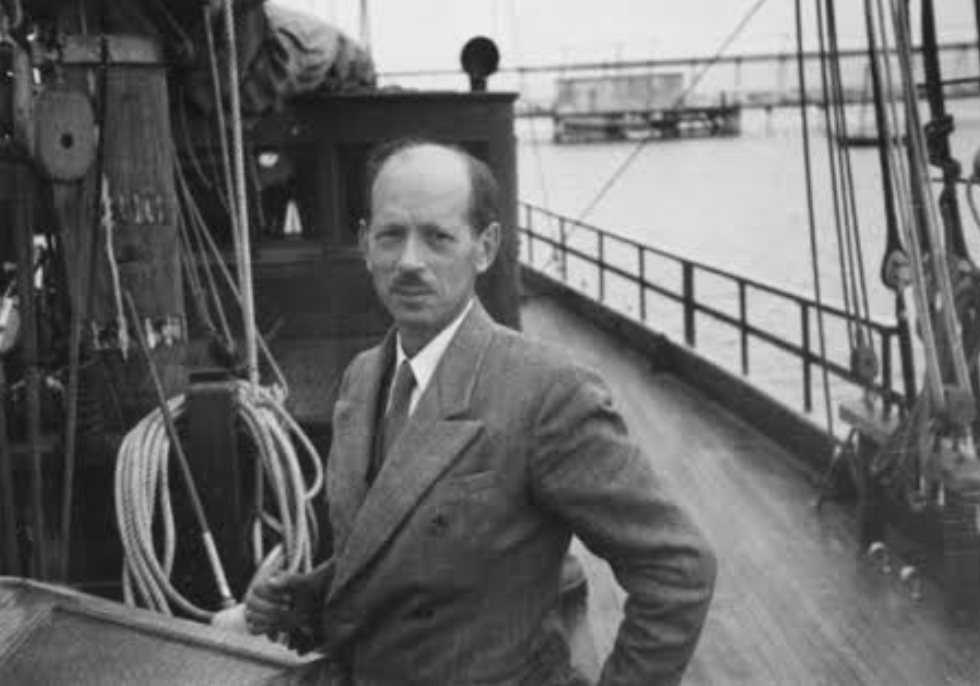
\includegraphics[width=0.40\textwidth]{Figures/Sverdrup.png}
    \caption{Harald Ulrik Sverdrup}
\end{figure}


% ============================================================
% ROSSBY
% ============================================================
\newpage
\section*{\underline{\textbf{Carl-Gustaf Arvid Rossby (1898--1957)}}}

\textbf{Nationality:} Swedish-American

\textbf{Generally known for:} Rossby was a meteorologist and physical geographer who became one of the central figures in modern atmospheric and geophysical fluid dynamics.

\textbf{Contribution to meteorology and oceanography:}

Rossby showed how the variation of the Coriolis parameter with latitude is fundamental to large-scale atmospheric and oceanic motion. The approximation

\[
f=f_0+\beta y \text{ where } \beta=\frac{df}{dy}.
\]

is called the beta-plane approximation. Rossby waves arise because large-scale meridional motion changes the planetary vorticity associated with Earth's rotation.

For a simple barotropic Rossby wave, the phase speed can be written

\[
c=U-\frac{\beta}{k^2+l^2}.
\]

If the background flow \(U\) is zero,

\[
c=-\frac{\beta}{k^2+l^2},
\]

so the wave propagates westward. Rossby waves explain major features of planetary-scale atmospheric circulation and are also important in ocean dynamics.

\begin{figure}[H]
    \centering
    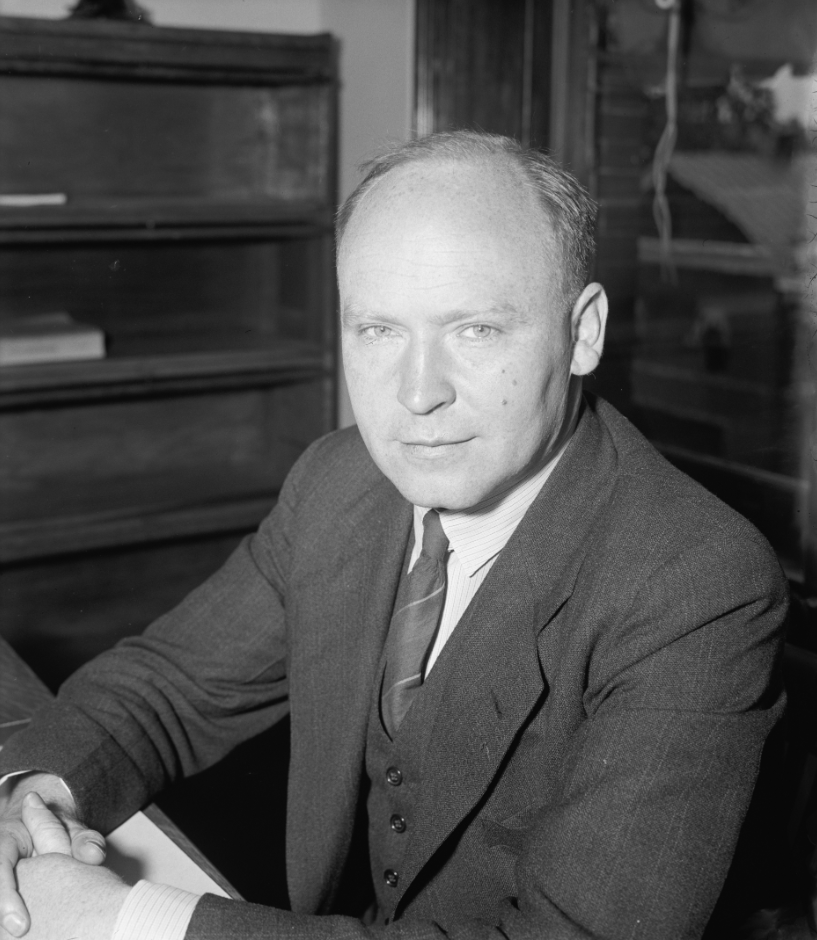
\includegraphics[width=0.30\textwidth]{Figures/Rossby.png}
    \caption{Carl-Gustaf Arvid Rossby}
\end{figure}


% ============================================================
% JACOB BJERKNES
% ============================================================
\newpage
\section*{\underline{\textbf{Jacob Aall Bonnevie Bjerknes (1897--1975)}}}

\textbf{Nationality:} Norwegian-American

\textbf{Generally known for:} Jacob Bjerknes was a meteorologist and one of the leading figures in the development of modern synoptic meteorology.

\textbf{Contribution to meteorology:}

Jacob Bjerknes developed the polar-front theory of midlatitude cyclones. He showed that extratropical cyclones are associated with strong temperature contrasts between different air masses. Along the boundary between these air masses, warm and cold fronts develop.

A developing cyclone can contain a warm sector between a warm front and a cold front. As the system evolves, the cold front can catch up with the warm front, producing an occluded front. This provided a physical interpretation of weather maps: fronts were not merely lines drawn between different weather conditions, but dynamically evolving boundaries between air masses. The Bergen school used these ideas to explain the life cycle of extratropical cyclones.

\begin{figure}[H]
    \centering
    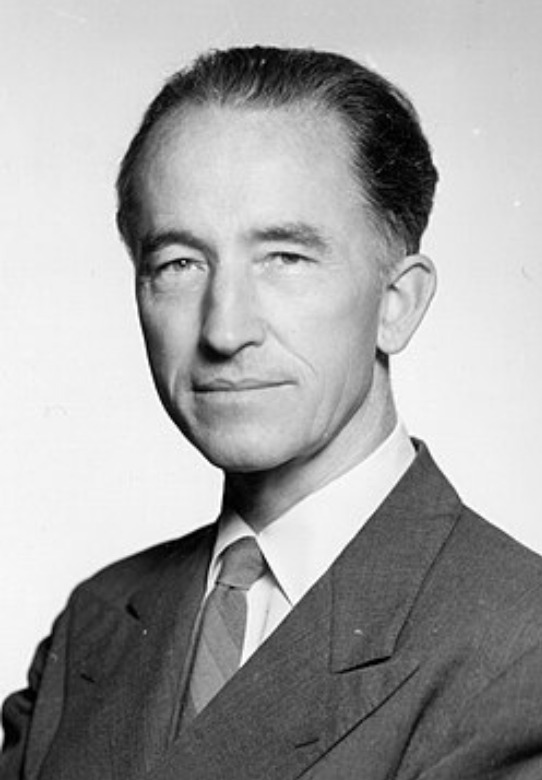
\includegraphics[width=0.30\textwidth]{Figures/Bjerknes2.png}
    \caption{Jacob Aall Bonnevie Bjerknes}
\end{figure}


% ============================================================
% KOLMOGOROV
% ============================================================
\newpage
\section*{\underline{\textbf{Andrey Nikolaevich Kolmogorov (1903--1987)}}}

\textbf{Nationality:} Russian / Soviet

\textbf{Generally known for:} Kolmogorov was a mathematician who made major contributions to probability theory, statistics, topology, information theory, and mathematical physics.

\textbf{Contribution to turbulence:}

Kolmogorov developed one of the most influential theories of turbulence. He proposed that at sufficiently small scales, turbulent motions become statistically universal and are controlled primarily by the energy dissipation rate $\varepsilon $ and the scale of the turbulent motion. His famous inertial-range energy spectrum is

\[
E(k)\propto
\varepsilon^{2/3}k^{-5/3},
\]

where \(k\) is wavenumber. The \(-5/3\) power law is one of the most recognizable signatures of a turbulent energy cascade.

Kolmogorov's theory describes how kinetic energy introduced at large scales can cascade toward smaller eddies until viscosity dissipates it as heat.

\begin{figure}[H]
    \centering
    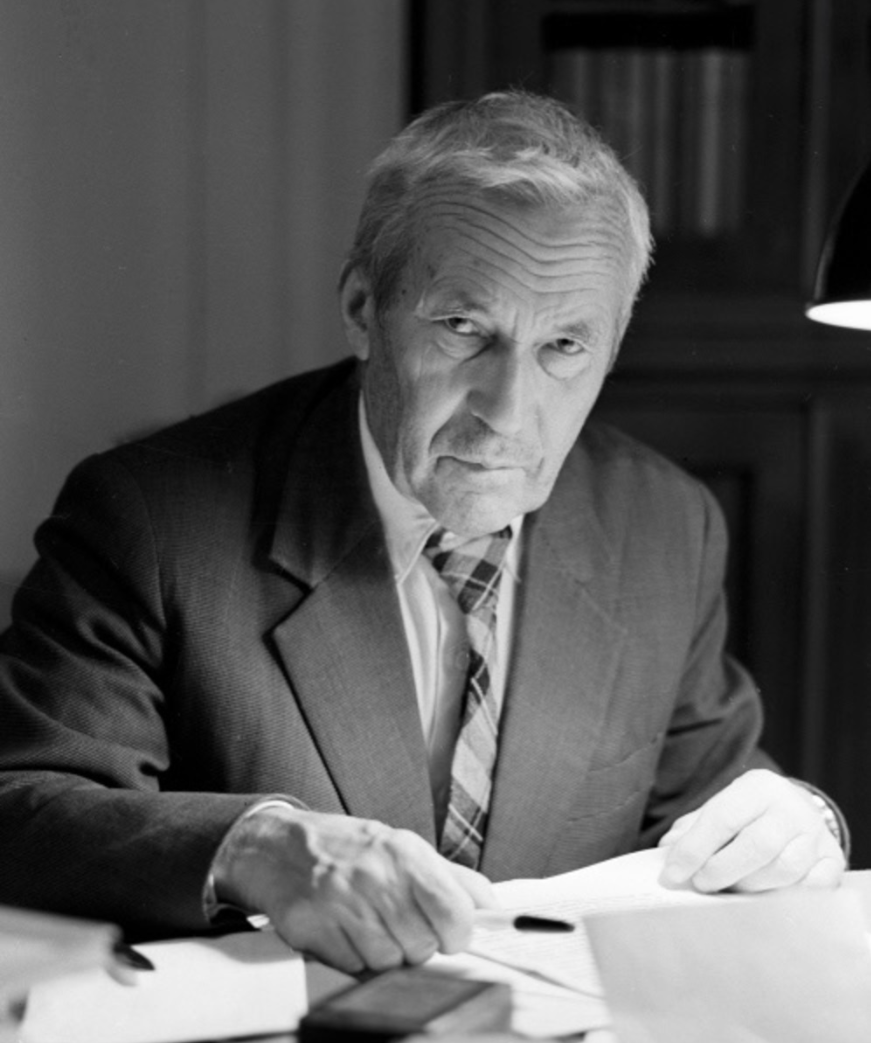
\includegraphics[width=0.30\textwidth]{Figures/Kolmogorov.png}
    \caption{Andrey Nikolaevich Kolmogorov}
\end{figure}


% ============================================================
% CHARNEY
% ============================================================
\newpage
\section*{\underline{\textbf{Jule Gregory Charney (1917--1981)}}}

\textbf{Nationality:} American

\textbf{Generally known for:} Charney was a meteorologist and geophysical fluid dynamicist who played a central role in modern numerical weather prediction.

\textbf{Contribution to meteorology:}

Charney developed mathematical theories that simplified the atmospheric equations while retaining the dominant large-scale dynamics. He was a major contributor to quasi-geostrophic theory, which describes large-scale atmospheric flow in which the pressure-gradient force and Coriolis force are approximately balanced. The geostrophic balance can be written schematically as

\[
f\mathbf{k}\times\mathbf{u}_g
=
-\frac{1}{\rho}\nabla_h p.
\]

Charney also led the first successful numerical weather prediction experiment in 1950. Using the newly developed electronic computer ENIAC, his group numerically integrated simplified atmospheric equations to forecast the evolution of a large-scale pressure pattern.

This demonstrated that Richardson's vision of numerical weather prediction was computationally possible.

\begin{figure}[H]
    \centering
    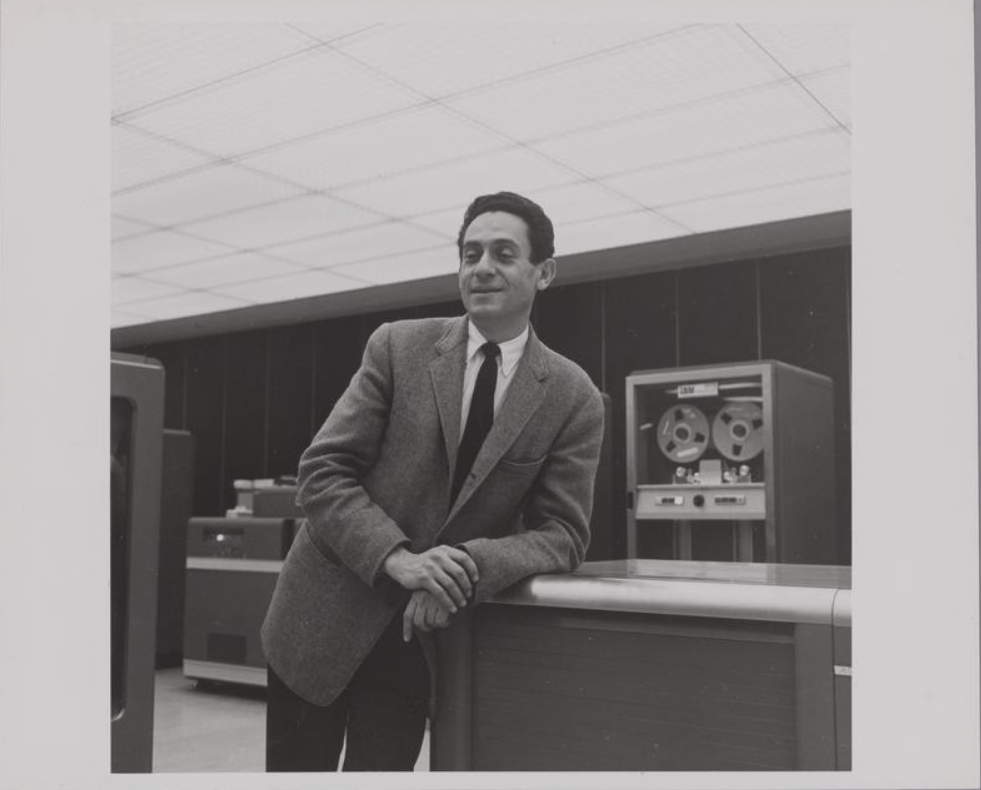
\includegraphics[width=0.45\textwidth]{Figures/Charney.png}
    \caption{Jule Gregory Charney}
\end{figure}


% ============================================================
% LORENZ
% ============================================================
\newpage
\section*{\underline{\textbf{Edward Norton Lorenz (1917--2008)}}}

\textbf{Nationality:} American

\textbf{Generally known for:} Lorenz was a mathematician and meteorologist who founded modern chaos theory in the context of atmospheric modelling.

\textbf{Contribution to meteorology:}

Lorenz discovered that deterministic atmospheric equations can produce extremely complicated and unpredictable behaviour. While studying a simplified model of convection, he obtained the system

\[
\frac{dx}{dt}
=
\sigma(y-x),
\]

\[
\frac{dy}{dt}
=
x(\rho-z)-y,
\]

\[
\frac{dz}{dt}
=
xy-\beta z.
\]

Although the equations are deterministic, tiny differences in the initial state can grow rapidly. This is called sensitive dependence on initial conditions.

Lorenz's work showed that there is a fundamental limit to long-range weather prediction: even if the governing equations are deterministic, imperfect knowledge of the initial atmospheric state can eventually produce very different forecasts. This became popularly associated with the phrase ``butterfly effect.''

\begin{figure}[H]
    \centering
    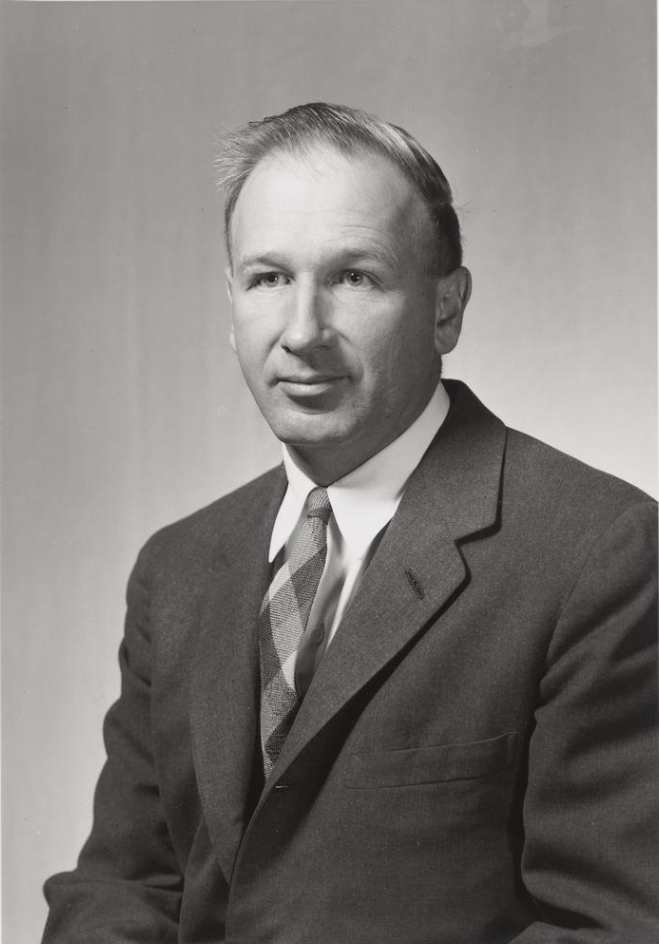
\includegraphics[width=0.30\textwidth]{Figures/Lorenz.png}
    \caption{Edward Norton Lorenz}
\end{figure}


% ============================================================
% STOMMEL
% ============================================================
\newpage
\section*{\underline{\textbf{Henry Melson Stommel (1920--1992)}}}

\textbf{Nationality:} American

\textbf{Generally known for:} Stommel was an oceanographer and physical oceanographer who made major contributions to the theory of ocean circulation.

\textbf{Contribution to physical oceanography:}

Stommel developed a theoretical explanation for why the circulation of subtropical ocean gyres becomes concentrated into strong western boundary currents. The key ingredients were the variation of the Coriolis parameter with latitude,

\[
f=f_0+\beta y,
\]

and friction.

His model showed that the ocean's response to wind forcing cannot remain spatially symmetric. Instead, the circulation becomes strongly concentrated near the western boundary. This provides the theoretical basis for the western intensification seen in real currents such as the Gulf Stream and Kuroshio.

Stommel's work was one of the major theoretical foundations of modern large-scale ocean circulation theory.

\begin{figure}[H]
    \centering
    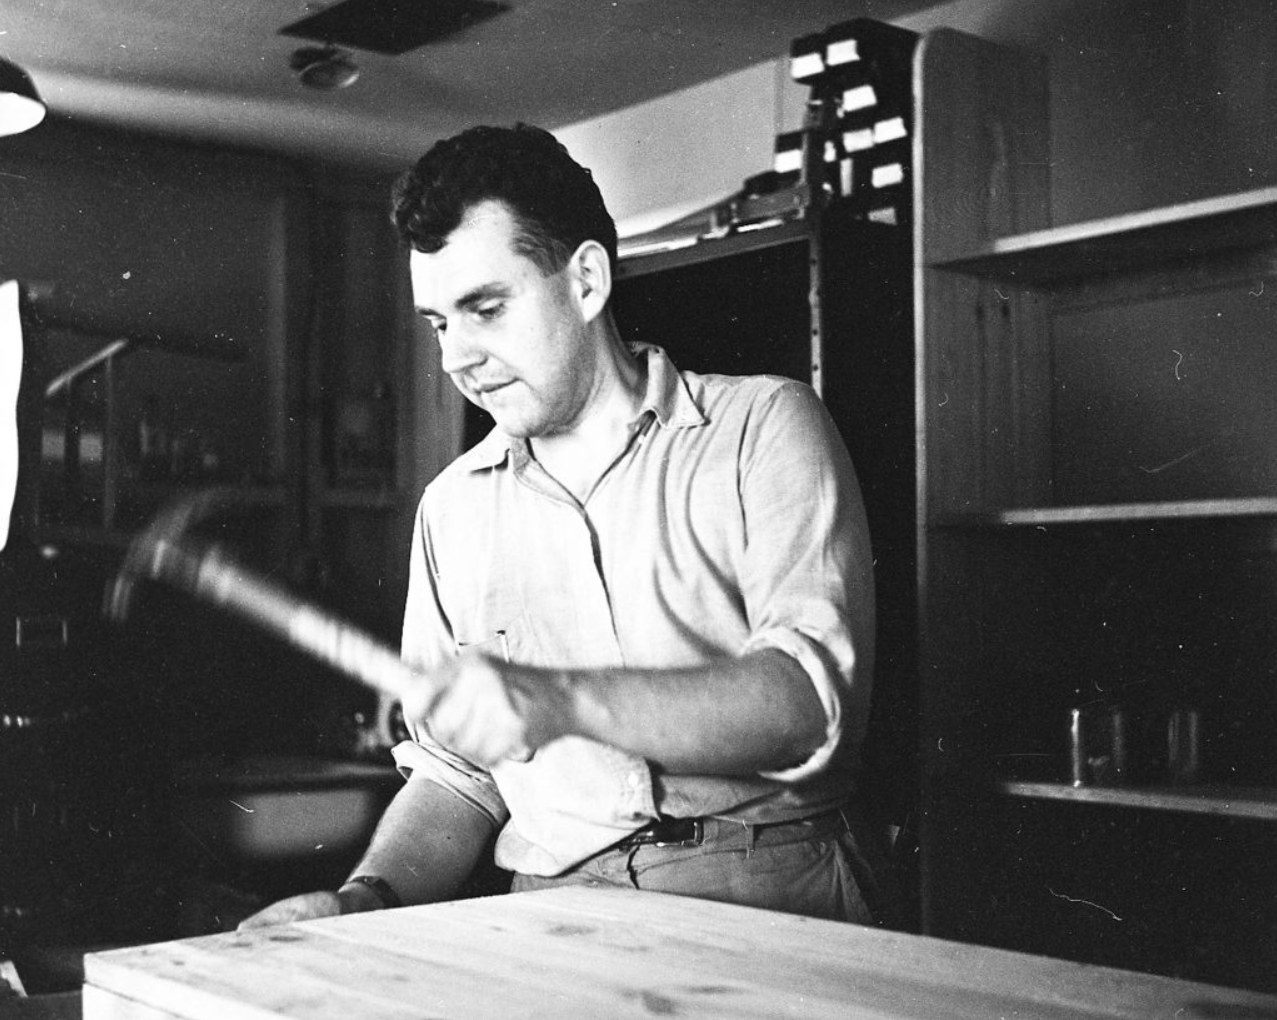
\includegraphics[width=0.45\textwidth]{Figures/Stommel.png}
    \caption{Henry Melson Stommel}
\end{figure}


% ============================================================
% SMAGORINSKY
% ============================================================
\newpage
\section*{\underline{\textbf{Joseph Smagorinsky (1924--2005)}}}

\textbf{Nationality:} American

\textbf{Generally known for:} Smagorinsky was a meteorologist and atmospheric scientist who was a pioneer of numerical climate and weather modelling.

\textbf{Contribution to atmospheric fluid dynamics:}

Smagorinsky developed an important model for representing turbulent motions that are too small to be resolved by a numerical atmospheric model. A weather or climate model divides the atmosphere into grid cells. Large turbulent structures can be explicitly represented, but smaller turbulent eddies occur below the grid scale.

Smagorinsky represented their effect using an effective turbulent viscosity. In simplified form,

\[
\nu_t\propto\Delta^2|S|,
\]

where \(\Delta\) is the grid or filter scale and \(|S|\) represents the magnitude of the resolved strain rate. This is the basis of the Smagorinsky subgrid-scale model.

The approach became extremely influential in numerical weather prediction, large-eddy simulation, and climate modelling because it provided a practical way of representing unresolved turbulence.

\begin{figure}[H]
    \centering
    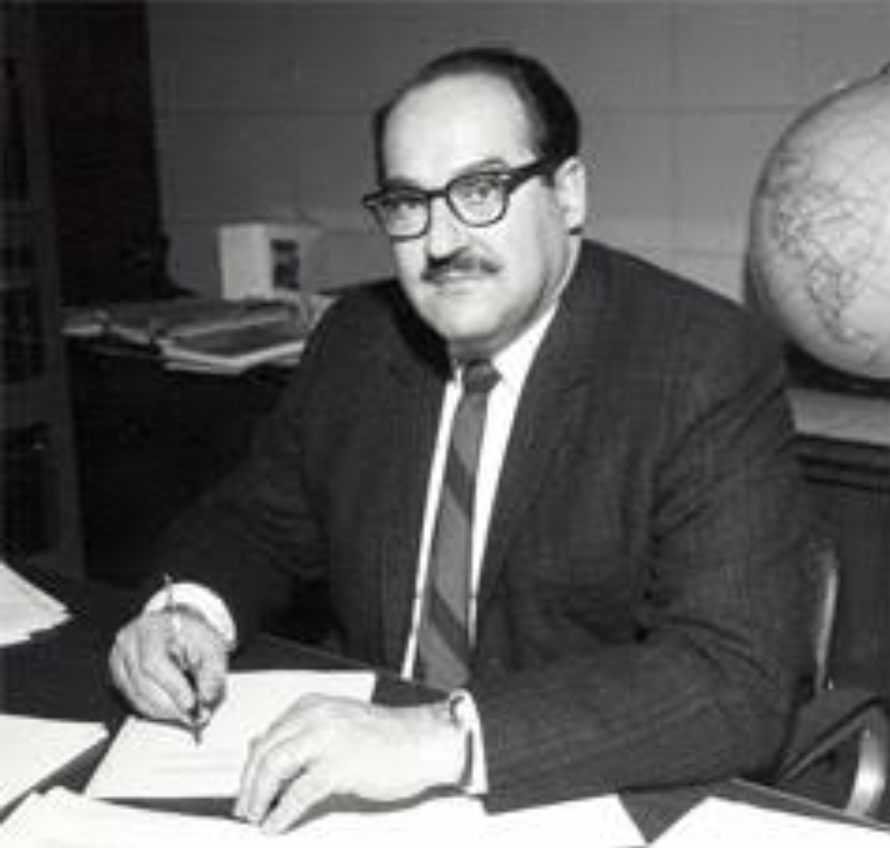
\includegraphics[width=0.40\textwidth]{Figures/Smagorinsky.png}
    \caption{Joseph Smagorinsky}
\end{figure}

\end{document}